\documentclass{article}
\usepackage[top=0.6in, bottom=1in, left=1.25in, right=1.25in]{geometry}

\usepackage{setspace}
\usepackage{xcolor}
\usepackage{hyperref}
\hypersetup{
    colorlinks=true,
    citecolor=black,
    linkcolor=black,
    urlcolor=black
}
\usepackage{amsmath,amssymb}
\usepackage{algorithm}
\usepackage{algorithmic}
\usepackage{tikz}
\usetikzlibrary{shapes.geometric, shapes.multipart, arrows.meta, positioning, calc, fit}
\usepackage{booktabs}
\usepackage{multirow}
\usepackage{graphicx}
\usepackage{enumitem}
\usepackage{caption}
\usepackage{array}
\usepackage{float}

\graphicspath{{figures/}}
\setlength{\emergencystretch}{3em}

\usepackage{etoolbox}
\AtBeginEnvironment{algorithmic}{\small}
\newcommand{\COMMENTR}[1]{\hfill $\triangleright$ #1}

\newcommand{\advlim}[3]{%
\begin{table}[H]
\centering
\caption{#1}
\small
\setstretch{1.2}
\renewcommand{\arraystretch}{1.3}
\setlength{\tabcolsep}{8pt}
\begin{tabular}{|>{\raggedright\arraybackslash}p{0.42\textwidth}|>{\raggedright\arraybackslash}p{0.42\textwidth}|}
\hline
\textbf{Advantages} & \textbf{Limitations} \\
\hline
\rule{0pt}{3.2ex}#2\vspace{5pt} & \rule{0pt}{3.2ex}#3\vspace{5pt} \\
\hline
\end{tabular}
\end{table}}

\title{\textbf{Adaptive Retransmission Scheduling in Underwater Acoustic Sensor Networks
based on ARQ\_HMAC}}
\author{}
\date{}

\begin{document}

\setstretch{1.5}

\maketitle
\vspace{-3.0em}

\section*{Team Members}

\noindent 1. 241CS209, Ankit Kumar, ankitkumar.241cs209@nitk.edu.in, 7295030513 \\
\noindent 2. 241CS239, Navadeep Sai K, navadeepsaikancharla.241cs239@nitk.edu.in, 8310029882 \\
\noindent 3. 241CS255, Shivam Kumar, shivam.241cs255@nitk.edu.in, 9234074220

% ══════════════════════════════════════════════════════════
%  ABSTRACT
% ══════════════════════════════════════════════════════════
\section*{Abstract}
{\setstretch{1.3}

Ocean monitoring, environmental research, deep-sea exploration, and surveillance all rely on Underwater Acoustic Sensor Networks (UASNs) to function. Because acoustic waves move slowly and the available bandwidth is quite narrow, underwater links end up dealing with very large propagation delays \cite{akyildiz2005,casari2011,jiang2018,kulla2022}. On top of that, whenever two or more nodes try to use the channel simultaneously, their packets crash into each other and have to be sent again, a process that burns through time, energy, and whatever little channel capacity exists \cite{casari2011,kulla2022,uwmac2007}. Our work takes ARQ\_HMAC \cite{dao2025} as a starting point. This is a hybrid MAC protocol that blends contention-based access with Automatic Repeat reQuest (ARQ) and pushes failed packets into collision-free TDMA slots for retransmission. The catch is that ARQ\_HMAC measures each node's propagation delay a single time during setup and then pads everything with a large fixed guard interval to stay safe against timing drift. But underwater conditions shift constantly and nodes move around after deployment, so that initial measurement quickly goes stale and the oversized guard ends up wasting valuable channel time \cite{casari2011,molinares2009}. What we propose, called Adaptive ARQ\_HMAC, fixes this by continuously refreshing the delay estimate using an exponentially weighted moving average paired with a change-detection threshold. It extracts timing information from time-tagged control frames, determines the size of the guard interval based on delay variance, schedules the TDMA slots based on actual packet arrivals, and fine-tunes the back-off algorithm according to the current level of contention. We coded both the original and the adaptive version inside the UnetStack simulator and ran 240 simulations across three scenarios: a static network, a 400~m network with moving AUVs, and a 3~km network with fast-moving AUVs. The adaptive technique leads to a reduction in the end-to-end delay by about 65--72\%, reduces the number of retransmissions by 44--47\%, collision rate by 23--30\%, while improving throughput by 6--23\% and packet delivery ratio by 3--12\%. All these benefits have statistical significance ($p < 0.001$).
\par}

\newpage

% ══════════════════════════════════════════════════════════
%  1. INTRODUCTION
% ══════════════════════════════════════════════════════════
\section{Introduction} \label{sec:intro}

\subsection{Background}
Over the past couple of decades, UASNs have grown into an essential piece of technology for a wide range of tasks: everything from gathering oceanographic data and keeping tabs on marine ecosystems to supporting offshore drilling operations, tsunami warning infrastructure, and naval defense \cite{akyildiz2005,casari2011}. The normal setup involves dispersing nodes with sensors on the seabed or attaching them to autonomous underwater vehicles (AUVs). The data collected is transmitted to the master node, which in turn transmits the data to a buoy on the surface or a research vessel. The big difference from the terrestrial wireless sensor networks most people are familiar with is the physical layer: radio-frequency (RF) signals get absorbed almost immediately in water, and optical signals scatter too much to be practical, so UASNs have to rely on acoustic waves instead \cite{akyildiz2005,jiang2018}.

And the acoustic channel is a very different beast from an RF channel. Sound moves through water at roughly 1500~m/s, about five orders of magnitude slower than electromagnetic waves travel through air. That means propagation delays can stretch from a few tens of milliseconds all the way to several seconds, depending on the distance between nodes \cite{akyildiz2005,kulla2022}. To put things in numerical perspective, by 400~m the delay is approximately 0.27~s and by 3~km it becomes 2~s, which actually exceeds the time needed for a packet transfer onto the link itself. Another challenge is bandwidth. It can be very limited and in most cases equals several kilohertz only, which value decreases even more with increasing range \cite{casari2011,jiang2018}. With data rates hovering in the kilobits-per-second range, every single packet hogs the channel for a noticeable chunk of time. All of this makes designing protocols for UASNs far more challenging than for their terrestrial counterparts \cite{akyildiz2005,kulla2022}. It is the MAC layer that lies at the very core of this issue since it controls access to the common acoustic medium by multiple nodes and has implications for throughput, delays, energy usage, and reliability \cite{jiang2018,kulla2022}.

\subsection{Challenges in Underwater Acoustic Sensor Networks}
The main reason building MAC and retransmission protocols for UASNs is so hard comes down to the hostile, ever-shifting nature of the underwater acoustic environment. The single biggest headache is the long and unpredictable propagation delay, which makes it nearly impossible to just port over the MAC or ARQ schemes that work fine on land \cite{akyildiz2005,slottedfama2006}. Because signals take so long to get from one place to another, there is a huge window of uncertainty where a sender simply has no idea what is going on at the receiver's end \cite{casari2011,kulla2022}. Carrier sensing, which works reasonably well in terrestrial Wi-Fi, becomes far less trustworthy underwater: a node might listen to the channel, hear nothing, and start transmitting, only for its packet to slam into another packet that was already in transit and just hadn't arrived yet. The result is a much higher collision rate than you would see on land \cite{casari2011}.

And once collisions start happening, the network has to retransmit, which drains battery power, inflates delays, and piles more traffic onto an already congested channel \cite{kulla2022,uwmac2007}. The narrow bandwidth amplifies the pain because each retransmission eats up a disproportionately large slice of the available capacity \cite{akyildiz2005,jiang2018}. Worse still, if the colliding nodes happen to wait the same amount of time before retrying, they will just collide again, potentially locking the network into a repeated failure loop. So the timing of retransmissions matters just as much as the decision to retransmit in the first place \cite{dao2025}.

On top of all that, the underwater channel is in a constant state of flux. Temperature gradients, salinity changes, ocean currents, reflections off the surface, and the movement of nodes or even passing marine life all conspire to alter the sound speed profile, multipath structure, and signal attenuation from one moment to the next \cite{casari2011,molinares2009}. These shifts directly affect how long it takes a signal to propagate and how reliable the link is \cite{casari2011,molinares2009}. Mobile platforms like AUVs and underwater gliders can change their distance to the gateway by hundreds of metres in a matter of minutes, meaning a delay measurement taken at deployment time might be completely wrong just a short while later \cite{cho2018}. And since underwater nodes run on batteries that are extremely difficult to swap out or recharge once deployed, squeezing every bit of efficiency out of the channel is not optional; it is a hard requirement \cite{kulla2022,uwmac2007}.

\subsection{Existing Approaches and Their Limitations}
Researchers have come up with quite a few MAC protocols for UASNs over the years, and they generally fall into three buckets: contention-free, contention-based, and hybrid \cite{jiang2018,kulla2022}. Contention-free schemes like TDMA and FDMA hand each node its own dedicated slice of the channel, which sounds clean in theory but in practice leads to poor utilization and demands tight synchronization, something that is notoriously hard to pull off given the enormous delays underwater \cite{akyildiz2005,jiang2018}. Contention-based protocols such as ALOHA and various CSMA flavors are more flexible and dodge the synchronization problem, but they tend to fall apart under heavy traffic because collisions skyrocket \cite{jiang2018,kulla2022}. Hybrid protocols try to get the best of both worlds by switching between the two modes depending on what the network looks like at any given moment \cite{dao2025,jiang2018}.

One of the more recent entries in this space is ARQ\_HMAC \cite{dao2025}, which pairs a contention-based CSMA phase for initial transmissions with a TDMA-based retransmission phase for recovery. After a collision, each involved node gets its own TDMA slot to retransmit, which neatly sidesteps the cascading collision problem that plagues purely contention-based designs and keeps throughput from collapsing as the load climbs. That said, ARQ\_HMAC, like most protocols in this category, leans on a one-time propagation delay estimate gathered during an initialization handshake. To absorb the inevitable timing errors that creep in later, it slaps on a large fixed guard time ($2t_d + t_{ACK}$) in both its acknowledgement timeout and its TDMA slot structure. The downside is that retransmission rounds drag on longer than they need to, pushing up end-to-end delay.

\subsection{Problem Statement}
The problem with the ARQ\_HMAC technique is that it calculates the propagation delay for each node to the master only once during the initial setup and then uses that static value to determine all subsequent acknowledgments' time-outs and TDMA transmission schedules. However, the underwater environment is dynamic. Channel conditions drift and nodes physically move, so the real delay can wander quite far from whatever was measured at the start. The protocol's way of coping is to build in conservative, fixed timing margins, which unfortunately waste channel time and inflate end-to-end delay. What this work sets out to do is make ARQ\_HMAC's retransmission scheduling responsive to the actual, evolving channel, so it stays correct when delays shift and gets faster when the delay is well understood.

\subsection{Objectives}
This project has three primary goals:
\begin{enumerate}
    \item Build an adaptive retransmission scheduling mechanism that continuously refreshes the propagation delay estimate using real-time feedback, replacing the single-shot estimation that ARQ\_HMAC relies on.
    \item Implement both the original ARQ\_HMAC protocol and the proposed adaptive variant inside the UnetStack simulation framework.
    \item Evaluate and compare the two approaches in terms of Packet Delivery Ratio (PDR), throughput, retransmission count, collision rate, and end-to-end delay across a range of traffic loads and channel conditions.
\end{enumerate}
Apart from the adaptive delay estimation presented in the previous progress report, the completed protocol additionally incorporates the better delay estimate for adjusting the guard time and arrangement of TDMA slots, as well as implements adaptive backoff scheme. All these modifications make use of the enhanced delay estimation for producing tangible gains in performance.

\subsection{Organization of the Report}
The rest of this report is organized as follows. The Related Work section is covered in Section~\ref{sec:lit_review}, which will begin with an historical overview in Section~\ref{sec:chronological}, followed by a more focused discussion of particular algorithms and their strengths and weaknesses in Section~\ref{sec:representative} and finally ending with a direct comparison in Section~\ref{sec:comparison}. The Proposed Adaptive ARQ\_HMAC is discussed in detail in Section~\ref{sec:proposed_approach}, which begins with an explanation of the architecture (Section~\ref{sec:architecture}), then algorithmic discussion (Section~\ref{sec:algorithm}) and finally rationale (Section~\ref{sec:justification}). The implementation within the UnetStack framework is discussed in Section~\ref{sec:implementation}, and the Results are covered in Section~\ref{sec:results}. Conclusions are drawn in Section~\ref{sec:conclusion}.

% ══════════════════════════════════════════════════════════
%  2. LITERATURE REVIEW
% ══════════════════════════════════════════════════════════
\section{Literature Review} \label{sec:lit_review}

In this section, we briefly review the various research lines in designing MAC and ARQ protocols for underwater acoustic sensor networks. We first present a brief chronology of the major works followed by an in-depth look at some exemplary algorithms.

\subsection{Existing Approaches in Chronological Order} \label{sec:chronological}

\textbf{Early works (2005--2009).} One of the first comprehensive looks at the research landscape for UASNs came from Akyildiz et al.~\cite{akyildiz2005}, who laid out the fundamental differences between terrestrial and underwater acoustic communication, especially the punishing propagation delays and the scarcity of bandwidth. Around the same time, Stojanovic~\cite{stojanovic2005} dug into ARQ for the underwater setting and showed that the classic stop-and-wait approach squanders most of the channel time just sitting around waiting for acknowledgements when delays are long. Her takeaway was that packet sizing and retransmission strategy need to be designed with the delay front and center. In 2006, Molins and Stojanovic~\cite{slottedfama2006} introduced Slotted FAMA, among the earliest handshaking MAC protocols tailored for underwater use. In the following year, there were many activities: Park and Rodoplu~\cite{uwmac2007} introduced a MAC protocol called UWAN-MAC based on energy-saving locally-scheduled protocol; Chirdchoo et al.~\cite{chirdchoo2007} investigated ALOHA-based schemes taking advantage of overheard messages to determine the distance between neighbours; and Peleato and Stojanovic~\cite{dacap2007} introduced DACAP, a handshaking procedure in which waiting times are adjusted according to distance between nodes. Syed et al.~\cite{tlohi2008} followed up in 2008 with T-Lohi, a contention protocol that fires off short tones to sense and count competing nodes before committing to a data transmission. Rounding out this early period, Molinares and Labrador~\cite{molinares2009} put forward a logical link layer protocol in 2009 that adjusts its transmission knobs based on observed channel quality.

\textbf{Intermediate developments (2010--2018).} Casari and Zorzi~\cite{casari2011} contributed an important theoretical treatment of the spatial-temporal uncertainty inherent in underwater channels and examined which design intuitions from terrestrial networking still hold up. In 2014, Chitre et al.~\cite{unetstack2014} released UnetStack, an agent-based protocol stack and simulator for underwater networks that we ended up using for this project. Also in 2014, Noh et al.~\cite{dots2014} proposed DOTS, a delay-aware opportunistic MAC that builds a map of propagation delays to neighbours from overheard traffic and uses that map to schedule concurrent transmissions, even when nodes are mobile. Cho et al.~\cite{cho2018} tackled the problem of asymmetric propagation delays in mobile scenarios and designed a TDMA scheme that accounts for the fact that the delay from A to B may differ from B to A. That same year, Jiang~\cite{jiang2018} published a broad survey of underwater MAC protocols organized around a reference model, noting a clear trend in the field toward hybrid designs.

\textbf{Recent advances (2019--2025).} Kulla et al.~\cite{kulla2022} delivered an updated survey that zooms in on the trade-offs between contention-based and contention-free approaches. Most recently, Dao and Tran~\cite{dao2025} introduced ARQ\_HMAC, which serves as the baseline for our work. It merges CSMA-style contention with TDMA-based collision-free retransmissions and demonstrates higher, more stable throughput than Pure ALOHA, ALOHA with CSMA, Slotted ALOHA, and Slotted ALOHA with CSMA, though it still depends on a static, one-shot delay estimate.

\textbf{Adaptive timers outside the underwater domain.} The problem of setting timeouts when the round-trip time is uncertain and drifting has been studied extensively in terrestrial networking. Jacobson's classic 1988 paper~\cite{jacobson1988} argued that a TCP retransmission timer should track both the average and the variability of the measured round-trip time, an idea that eventually made its way into RFC~6298~\cite{rfc6298}. Similarly, the binary exponential backoff mechanism in IEEE~802.11~\cite{ieee80211} dynamically adjusts the contention window based on how much contention the node is actually seeing. Both of these ideas find their way into the protocol we propose.

\subsection{Representative Algorithms, with Pros and Cons} \label{sec:representative}
Here we take a closer look at six representative protocols. For each one, we outline how it works and then weigh its strengths against its weaknesses. The goal is to pinpoint the specific gaps that our proposed mechanism tries to fill.

\subsubsection{Slotted FAMA}
Slotted Floor Acquisition Multiple Access~\cite{slottedfama2006} uses an RTS/CTS protocol where time is divided into slots whose duration corresponds to the maximum propagation delay plus one control packet. Transmissions are only allowed at the beginning of the slot. The node first sends an RTS and awaits a response in the form of a CTS after which it sends the payload data. One benefit of this scheme is that data packets are collision-free as the collision takes place between the control packets. This is illustrated in Algorithm~\ref{alg:fama} and Table~\ref{tab:fama} below.

\begin{algorithm}[H]
\caption{Slotted FAMA (sender side)}
\label{alg:fama}
\begin{algorithmic}[1]
\STATE wait for the start of the next slot
\STATE send RTS to the receiver
\IF{CTS received within the following slot}
    \STATE send DATA at the start of the next slot
    \STATE wait for ACK
\ELSE
    \STATE back off for a random number of slots and go to line 1
\ENDIF
\end{algorithmic}
\end{algorithm}

\advlim{Advantages and limitations of Slotted FAMA.\label{tab:fama}}
{Gets rid of data packet collisions entirely and provides reasonably fair channel access among competing nodes. Synchronizing to slot boundaries means the handshake does not depend on knowing the exact propagation delay.}
{Each slot has to be long enough for the maximum propagation delay, which kills channel utilization. Every data packet triggers a full handshake, an expensive proposition when delays are large, and any retransmission requires going through the whole handshake again.}

\subsubsection{UWAN-MAC}
UWAN-MAC~\cite{uwmac2007} focuses on energy first, in which each node determines its own transmission schedule and shares it with neighbouring nodes, who will remain in sleep mode unless there is a transmission known. It does not use global synchronization but rather focuses on passive channel listening for coordination purposes (refer to Table~\ref{tab:uwan}).

\advlim{Advantages and limitations of UWAN-MAC.\label{tab:uwan}}
{Extremely energy-efficient because it cuts idle listening to a minimum and sidesteps the overhead of global clock synchronization.}
{Has no real mechanism for resolving collisions on the fly: if multiple nodes end up with overlapping schedules, they can keep colliding over and over. There is also no adaptive handling of delay changes for retransmission scheduling.}

\subsubsection{T-Lohi}
In T-Lohi~\cite{tlohi2008}, a contention algorithm, the transmitting node sends out a tone when it wishes to send data. The number of tones heard by the nodes will give them an estimate of the number of competing nodes, and they will then defer transmission. These trade-offs have been summarized in Table~\ref{tab:tlohi}.

\advlim{Advantages and limitations of T-Lohi.\label{tab:tlohi}}
{The short tones make contention cheap and give nodes a direct read on the current load, which helps keep data packet collisions down.}
{Contention rounds need to last at least as long as the maximum propagation delay, which throttles throughput in larger networks. When a packet is lost, it just goes back through the same contention process; there is no dedicated collision-free retransmission phase.}

\subsubsection{DOTS}
DOTS~\cite{dots2014} is a delay-sensitive opportunistic MAC. The nodes keep learning about the delays to their neighbors through the use of timestamps received from overheard packets and then use the delay map to schedule transmission times that do not collide with any of the receivers regardless of other ongoing transmissions. Refer to Table~\ref{tab:dots} below for more details.

\advlim{Advantages and limitations of DOTS.\label{tab:dots}}
{Uses the lengthy propagation delay to its advantage by allowing concurrent transmissions rather than working against it. The delay map is kept up-to-date using overheard traffic, which can deal with mobility fairly well.}
{Demands synchronized clocks and a significant amount of per-node state. Scheduling decisions get complicated fast as the neighbour count grows. There is also no structured retransmission phase for when collisions do happen.}

\subsubsection{Asymmetric Propagation Delay-Aware TDMA}
Cho et al.~\cite{cho2018} introduced an asymmetric TDMA scheme that takes into consideration the asymmetric nature of the delay encountered while traveling from the sender to the receiver in mobile underwater environments (see Table~\ref{tab:asym}).

\advlim{Advantages and limitations of Asymmetric Delay-Aware TDMA.\label{tab:asym}}
{Handles mobility and delay asymmetry problem, hence providing more precise scheduling under dynamic environment than the conventional TDMA algorithm.}
{Delay adjustments happen at fixed intervals, so a sudden change between two updates can still throw off slot alignment. And like any pure TDMA scheme, it leaves slots sitting empty when the traffic load is light.}

\subsubsection{ARQ\_HMAC}
ARQ\_HMAC~\cite{dao2025} is a hybrid MAC that uses asynchronous CSMA for first-time transmissions and switches to synchronous TDMA for retransmissions. During an initialization phase, every node measures its propagation delay $t_{D_i}$ to the master. When the master spots a collision, it broadcasts a negative acknowledgement (NACK), and each node then figures out when a common TDMA period starts based on its delay estimate and retransmits in its assigned slot, avoiding repeat collisions with the same interferer. Both the timeout and the TDMA slots include a fixed guard time $t_{guard} = 2t_d + t_{ACK}$. The protocol's phases and timing equations are spelled out in Section~III of~\cite{dao2025}; Section~\ref{sec:architecture} identifies the specific quantities our proposed protocol modifies. Table~\ref{tab:arqhmac} lays out the pros and cons.

\advlim{Advantages and limitations of ARQ\_HMAC.\label{tab:arqhmac}}
{Maintains consistent throughput performance regardless of network load since TDMA retransmissions overcome the collisions that occur in entirely contention-based protocols, while random access remains efficient with light network loads.}
{Propagation delay is calculated only once and is not modified to reflect changes in the environment and movement of nodes. The fixed guard period of $2t_d + t_{ACK}$ inflates timeouts and TDMA slots, and TDMA retransmissions receive no acknowledgment.}

\subsection{Comparison of the Approaches} \label{sec:comparison}
Table~\ref{tab:comparison} gives a comparison of the schemes under consideration, while Figure~\ref{fig:mac_classification} shows their position in the wider taxonomy. Up till now, delay awareness and collision-free retransmission have mostly been addressed independently. DOTS and Asym-TDMA are both delay aware but lack a formalized retransmission stage. ARQ\_HMAC, in turn, ensures collision free retransmission but uses a fixed delay value. Current state-of-the-art protocols do not combine (i) collision-free retransmission, (ii) dynamic delay estimation, and (iii) time margins calculated based on delay variance. Our proposed Adaptive ARQ\_HMAC aims at filling that gap.

\begin{table}[H]
\centering
\caption{Comparison of the reviewed schemes.}
\label{tab:comparison}
\small
\setstretch{1.1}
\begin{tabular}{@{}>{\raggedright\arraybackslash}p{2.6cm} l
>{\raggedright\arraybackslash}p{4.3cm}
>{\raggedright\arraybackslash}p{4.3cm}@{}}
\toprule
Scheme & Year & Pros & Cons \\
\midrule
Slotted FAMA~\cite{slottedfama2006} & 2006 & No data collisions, fair access & Long slots, handshake per packet \\
UWAN-MAC~\cite{uwmac2007} & 2007 & Energy efficient & Repeated collisions at high load \\
T-Lohi~\cite{tlohi2008} & 2008 & Cheap tone-based contention & Long contention rounds \\
DOTS~\cite{dots2014} & 2014 & Delay map, concurrent transmissions, mobility & Complex, no retransmission phase \\
Asym-TDMA~\cite{cho2018} & 2018 & Handles mobility and asymmetry & Periodic updates, idle slots \\
ARQ\_HMAC~\cite{dao2025} & 2025 & Stable throughput, collision-free retransmission & Static delay estimate, fixed guard \\
\textbf{Adaptive ARQ\_HMAC (proposed)} & N/A & Continuous delay tracking, adaptive guard and slots, adaptive backoff & Needs clock synchronisation; TDMA retransmissions unacknowledged \\
\bottomrule
\end{tabular}
\end{table}

\begin{figure}[H]
\centering
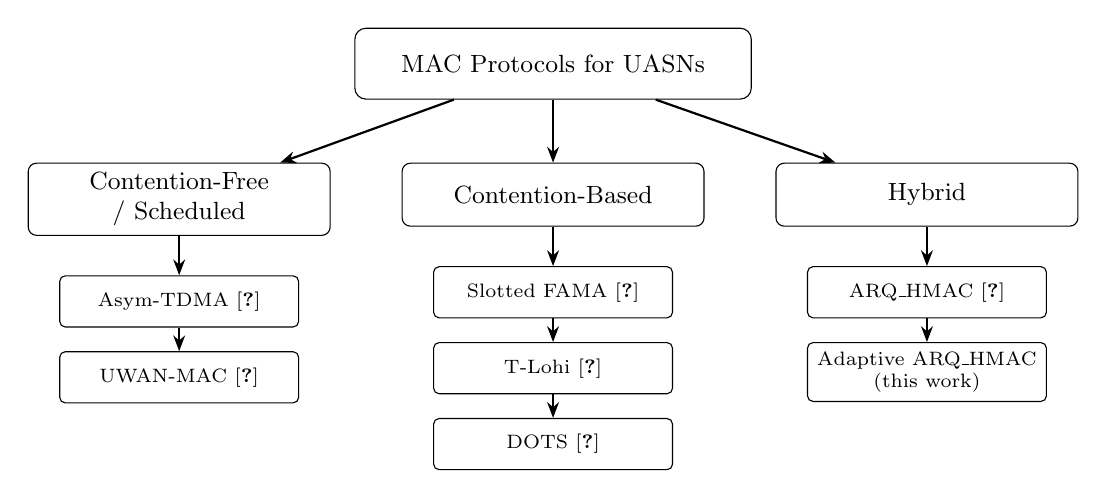
\begin{tikzpicture}[
    box/.style={rectangle, draw=black, fill=white, text width=3.6cm,
                minimum height=0.8cm, align=center, rounded corners=3pt, font=\small},
    root/.style={rectangle, draw=black, fill=white, text width=4.8cm,
                 minimum height=0.9cm, align=center, rounded corners=4pt, font=\small},
    leaf/.style={rectangle, draw=black, fill=white, text width=2.8cm,
                 minimum height=0.65cm, align=center, rounded corners=2pt, font=\scriptsize},
    arr/.style={-{Stealth[length=2mm]}, thick, draw=black}
]
\node[root] (mac) {MAC Protocols for UASNs};
\node[box, below left=0.8cm and 0.3cm of mac] (cf) {Contention-Free / Scheduled};
\node[box, below=0.8cm of mac] (cb) {Contention-Based};
\node[box, below right=0.8cm and 0.3cm of mac] (hy) {Hybrid};
\draw[arr] (mac) -- (cf); \draw[arr] (mac) -- (cb); \draw[arr] (mac) -- (hy);
\node[leaf, below=0.5cm of cf] (tdma) {Asym-TDMA~\cite{cho2018}};
\node[leaf, below=0.3cm of tdma] (uwan) {UWAN-MAC~\cite{uwmac2007}};
\draw[arr] (cf) -- (tdma); \draw[arr] (tdma) -- (uwan);
\node[leaf, below=0.5cm of cb] (fama) {Slotted FAMA~\cite{slottedfama2006}};
\node[leaf, below=0.3cm of fama] (tl) {T-Lohi~\cite{tlohi2008}};
\node[leaf, below=0.3cm of tl] (dots) {DOTS~\cite{dots2014}};
\draw[arr] (cb) -- (fama); \draw[arr] (fama) -- (tl); \draw[arr] (tl) -- (dots);
\node[leaf, below=0.5cm of hy] (arq) {ARQ\_HMAC~\cite{dao2025}};
\node[leaf, below=0.3cm of arq] (prop) {Adaptive ARQ\_HMAC (this work)};
\draw[arr] (hy) -- (arq); \draw[arr] (arq) -- (prop);
\end{tikzpicture}
\caption{Classification of MAC protocols for underwater acoustic sensor networks.}
\label{fig:mac_classification}
\end{figure}

% ══════════════════════════════════════════════════════════
%  3. PROPOSED APPROACH
% ══════════════════════════════════════════════════════════
\section{Proposed Approach} \label{sec:proposed_approach}

\subsection{Architecture} \label{sec:architecture}

\paragraph{What the proposal changes.} Our protocol leaves the overall structure of ARQ\_HMAC untouched: the phases, frame types, and operating rules described in Section~III of~\cite{dao2025} all stay the same. That includes the initial phase (Eqs.~(1)--(2) of~\cite{dao2025}), the CSMA phase with its ACK/NACK exchange, the unacknowledged TDMA retransmission phase, and the TDMA period of $n\,t_{slot}$ (Eqs.~(9)--(10) of~\cite{dao2025}). The only things we touch are the quantities listed in Table~\ref{tab:changes}. In the original ARQ\_HMAC, the delay $t_{D_i}$ gets measured a single time and then never updated. The guard interval $2t_d + t_{ACK}$ adds up to around a whole packet time's worth of additional overhead, and each TDMA timeslot also sets aside $t_{max}$ in order to accommodate propagation delay spread. To put into perspective how much overhead this is: at a distance of 3~km, where $t_d = 1$~second and $t_{max} = 2$~seconds, one TDMA timeslot will be 4.1~seconds long, but only a second of that time contains any real information.

\begin{table}[H]
\centering
\caption{Quantities of ARQ\_HMAC that the proposed protocol changes; [1, Eq.~$k$] refers to the equations of~\cite{dao2025}. Everything else is unchanged.}
\label{tab:changes}
\small
\setstretch{1.1}
\begin{tabular}{@{}>{\raggedright\arraybackslash}p{3.9cm}>{\raggedright\arraybackslash}p{3.5cm}>{\raggedright\arraybackslash}p{4.8cm}@{}}
\toprule
\textbf{Quantity} & \textbf{ARQ\_HMAC} & \textbf{Adaptive ARQ\_HMAC} \\
\midrule
Delay $t_{D_i}$ \cite[Eq.~2]{dao2025} & measured once in the initial phase & initial value from \cite[Eq.~2]{dao2025}, then $t^{sched}_{D_i}$ updated continuously, Eqs.~(\ref{eq:ewma})--(\ref{eq:timestamp}) \\
Guard $t_{guard}$ \cite[Eq.~4]{dao2025} & $2t_d + t_{ACK}$ & $t_{guard,i}$ from the measured deviation, Eq.~(\ref{eq:guard}) \\
ACK timeout \cite[Eq.~3]{dao2025} & $2t_{D_i} + t_{guard}$ & $2t^{sched}_{D_i} + t_{guard,i}$ \\
TDMA start \cite[Eq.~5]{dao2025} & uses $t_{D_i}$ & uses $t^{sched}_{D_i}$ \\
Slot width $t_{slot}$ \cite[Eq.~6]{dao2025} & $t_{max} + t_{guard}$ & $t_{guard}$, set by the master and announced in the NACK \\
Slot start $t_{slot_i}$ \cite[Eq.~7]{dao2025} & transmission at slot start & arrival at slot start, Eq.~(\ref{eq:aligned}) \\
Channel access & transmit as soon as the channel is free & adaptive random backoff \\
\bottomrule
\end{tabular}
\end{table}

\paragraph{Proposed architecture.} Here we present five novel methods that have been illustrated in Figure~\ref{fig:architecture} below, namely: (1) adaptive delay estimation coupled with change detection, (2) delay measurement through timestamps in the master frames, (3) adaptive guard period, (4) aligned TDMA slots and (5) adaptive backoff. The first two methods cooperate in order to ensure that the estimate of the delay is always up-to-date. The rest use this to improve their performance.

\begin{figure}[H]
\centering
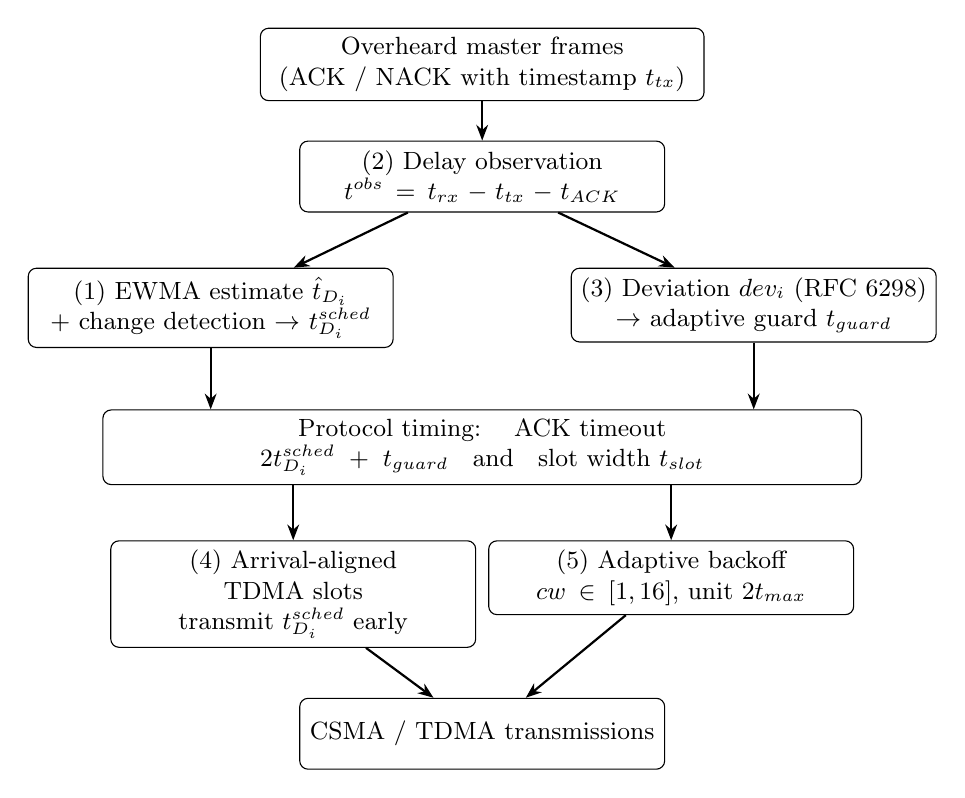
\begin{tikzpicture}[
    blk/.style={rectangle, draw=black, fill=white, text width=4.4cm, minimum height=0.9cm,
                align=center, rounded corners=3pt, font=\small},
    hl/.style={blk},
    arr/.style={-{Stealth[length=2mm]}, thick, draw=black}
]
\node[blk, text width=5.4cm] (frames) {Overheard master frames\\(ACK / NACK with timestamp $t_{tx}$)};
\node[hl, below=0.5cm of frames] (obs) {(2) Delay observation\\$t^{obs} = t_{rx} - t_{tx} - t_{ACK}$};
\node[hl, below left=0.7cm and -1.2cm of obs] (ewma) {(1) EWMA estimate $\hat t_{D_i}$\\+ change detection $\rightarrow t^{sched}_{D_i}$};
\node[hl, below right=0.7cm and -1.2cm of obs] (guard) {(3) Deviation $dev_i$ (RFC 6298)\\$\rightarrow$ adaptive guard $t_{guard}$};
\node[blk, below=2.5cm of obs, text width=9.4cm] (timing) {Protocol timing: \; ACK timeout $2t^{sched}_{D_i} + t_{guard}$ \; and \; slot width $t_{slot}$};
\node[hl, anchor=north] (slots) at ($(timing.south)+(-2.4,-0.7)$) {(4) Arrival-aligned TDMA slots\\transmit $t^{sched}_{D_i}$ early};
\node[hl, anchor=north] (bo) at ($(timing.south)+(2.4,-0.7)$) {(5) Adaptive backoff\\$cw \in [1, 16]$, unit $2t_{max}$};
\node[blk, anchor=north] (mac) at ($(timing.south)+(0,-2.7)$) {CSMA / TDMA transmissions};
\draw[arr] (frames) -- (obs);
\draw[arr] (obs) -- (ewma);
\draw[arr] (obs) -- (guard);
\draw[arr] (ewma) -- (ewma |- timing.north);
\draw[arr] (guard) -- (guard |- timing.north);
\draw[arr] (slots |- timing.south) -- (slots);
\draw[arr] (bo |- timing.south) -- (bo);
\draw[arr] (slots) -- (mac);
\draw[arr] (bo) -- (mac);
\end{tikzpicture}
\caption{Architecture of Adaptive ARQ\_HMAC. Blocks numbered (1)--(5) are the added mechanisms.}
\label{fig:architecture}
\end{figure}

\paragraph{(1) Adaptive delay estimate with change detection.} Building on what we outlined in the progress report, each sensor maintains a running estimate $\hat{t}_{D_i}$. We seed it with the value measured during the initial phase (Eq.~(2) of~\cite{dao2025}) and then refresh it every time a new observation comes in, using an Exponentially Weighted Moving Average (EWMA):
\begin{equation}
\hat{t}_{D_i}^{(k)} = \alpha \cdot t_{D_i}^{\text{obs},(k)} + (1 - \alpha) \cdot \hat{t}_{D_i}^{(k-1)}.
\label{eq:ewma}
\end{equation}
We do not want the protocol to recalculate its entire schedule every time the estimate jitters by a millisecond or two, so the value that actually feeds into the timing logic, $t_{D_i}^{\text{sched}}$, only gets replaced when the drift crosses a threshold $\theta$:
\begin{equation}
\Delta_i^{(k)} = \left| \hat{t}_{D_i}^{(k)} - t_{D_i}^{\text{sched}} \right| > \theta
\;\Rightarrow\; t_{D_i}^{\text{sched}} \leftarrow \hat{t}_{D_i}^{(k)},
\label{eq:deviation}
\end{equation}
at which point the ACK timeout and the TDMA schedule (Eqs.~(3) and (5)--(7) of~\cite{dao2025}) are recomputed using the fresh $t_{D_i}^{\text{sched}}$. In our setup we chose $\theta = 5$~ms and $\alpha = 0.7$. The relatively high $\alpha$ puts more weight on the latest observation, which makes sense for a node that may have moved a fair bit between two consecutive measurements.

\paragraph{(2) Timestamped delay observations.} In the progress report version, a delay observation came from the round trip of a node's own data packet and its ACK: $t_{D_i}^{\text{obs}} = (t_{\text{ACK\_recv}} - t_{\text{data\_send}} - t_d - t_{ACK})/2$. The problem is that under moderate traffic a node might only see its own ACK once every minute or two, so the estimate falls behind quickly when the node is on the move. Fortunately, ARQ\_HMAC already assumes that all nodes share a common time reference after the initial phase (the operating phase starts at $t = 0$ for everyone~\cite{dao2025}). We take advantage of this by having the master stamp the transmission start time $t_{tx}$ into every ACK and NACK it sends, and by broadcasting ACKs with the destination address tucked into the payload so that every sensor in range can overhear them. Whenever a sensor receives a master frame at time $t_{rx}$ (measured at the end of reception), it can extract a one-way delay observation:
\begin{equation}
t_{D_i}^{\text{obs}} = t_{rx} - t_{tx} - t_{ACK}.
\label{eq:timestamp}
\end{equation}
In our simulations this trick gives each sensor roughly 130 observations per 30-minute run at moderate load, compared to about one per own ACK. The idea is not new: DOTS~\cite{dots2014} maintains its delay map in essentially the same way.

\paragraph{(3) Adaptive guard time.} The guard interval has to cover the actual duration of the data and ACK frames ($t_d + t_{ACK}$) plus whatever uncertainty remains in the delay estimate. Rather than hard-coding an extra margin of one full data-packet time, we measure the uncertainty on the fly, borrowing the approach TCP uses to track round-trip time variation~\cite{jacobson1988,rfc6298}:
\begin{equation}
dev_i \leftarrow (1-\beta)\, dev_i + \beta \left| t_{D_i}^{\text{obs}} - \hat{t}_{D_i} \right|,
\qquad
t_{guard,i} = t_d + t_{ACK} + \max\left(t_{ACK},\; 2K\, dev_i\right),
\label{eq:guard}
\end{equation}
using the standard RFC~6298 constants $\beta = 1/4$ and $K = 4$. We initialize the deviation at $dev_i = t_d/(2K)$, which conveniently reproduces the original paper's guard of $2t_d + t_{ACK}$ right out of the gate. From there, the guard only shrinks as the measurements confirm that the delay is behaving predictably; if the delay starts jumping around, $dev_i$ climbs and the guard swells back toward the conservative ARQ\_HMAC values. Since all nodes in a TDMA round must agree on the same slot size, each sensor piggybacks its $dev_i$ inside its data packets, and the master picks a slot width large enough for the least predictable sensor and broadcasts that width in every NACK.

\paragraph{(4) Arrival-aligned TDMA slots.} In the original ARQ\_HMAC, every node fires off its retransmission at the very start of its assigned slot (Eq.~(7) of~\cite{dao2025}). The packet then takes up to $t_{max}$ to reach the master, which is why each slot has to reserve $t_{max}$ for propagation spread. We flip this around: in our version, a slot defines the window during which the packet \emph{arrives} at the master, and node $i$ transmits $t_{D_i}^{\text{sched}}$ earlier to compensate ($t_{start\_TDMA}$ is still computed as in Eq.~(5) of~\cite{dao2025}, just with $t^{sched}_{D_i}$ plugged in):
\begin{equation}
t_{arrive} = t_{start\_TDMA} + t_{max}, \qquad
t_{slot_i} = t_{arrive} + n_i\, t_{slot} - t_{D_i}^{\text{sched}}, \qquad
t_{slot} = t_{guard}.
\label{eq:aligned}
\end{equation}
The upshot is that packets land back to back at the master and each slot shrinks by the full $t_{max}$: at 400~m the slot drops from 2.37~s to roughly 1.2~s, and at 3~km it goes from 4.1~s down to about 1.3~s. This only works because the delay estimate is accurate enough to trust.

\paragraph{(5) Adaptive backoff.} When a TDMA round wraps up, every node that still has queued packets jumps back into CSMA at the same instant. Nodes that had been holding off because the channel was busy also rush to transmit the moment it clears. A synchronized transmission burst is achieved and, needless to say, a new set of collisions occurs. In order to destroy synchronization, each node will wait for a random time chosen uniformly from $[0,\; cw \cdot 2t_{max}]$. The unit $2t_{max}$ corresponds to the longest possible propagation time between any two sensors, which means the first node to start transmitting will be heard by the others before their backoff timers expire. The contention window $cw$ follows the binary exponential backoff rule from IEEE~802.11~\cite{ieee80211}: it doubles after every NACK or timeout, caps out at 16, and resets to 1 following a successful ACK.

\subsection{Algorithm} \label{sec:algorithm}
Algorithm~\ref{alg:adaptive} describes only those parts that are added or changed in the sensor with ARQ\_HMAC, while all the rest is done as described in~\cite{dao2025}. This expands upon the Algorithm~1 described in the progress report. These new steps are incorporated into the control flow of the sensor as shown in Figure~\ref{fig:adaptive_flowchart}.

\begin{algorithm}[H]
\caption{Changes to a sensor of ARQ\_HMAC (sensor $i$)}
\label{alg:adaptive}
\begin{algorithmic}[1]
\REQUIRE $t_{D_i}^{(0)}$ from the initial phase of ARQ\_HMAC, $\alpha$, $\theta$, $\beta$, $K$
\STATE $\hat{t}_{D_i} \leftarrow t_{D_i}^{(0)}$; \; $t_{D_i}^{\text{sched}} \leftarrow t_{D_i}^{(0)}$; \; $dev_i \leftarrow t_d/(2K)$; \; $cw \leftarrow 1$ \COMMENTR{new state}
\FOR{each master frame (ACK or NACK, any destination) received} 
    \STATE $t^{\text{obs}} \leftarrow t_{rx} - t_{tx} - t_{ACK}$ \COMMENTR{Eq.~(\ref{eq:timestamp})}
    \STATE $dev_i \leftarrow (1-\beta)\,dev_i + \beta\,|t^{\text{obs}} - \hat{t}_{D_i}|$; update $t_{guard,i}$ \COMMENTR{Eq.~(\ref{eq:guard})}
    \STATE $\hat{t}_{D_i} \leftarrow \alpha\, t^{\text{obs}} + (1-\alpha)\,\hat{t}_{D_i}$ \COMMENTR{Eq.~(\ref{eq:ewma})}
    \IF{$|\hat{t}_{D_i} - t_{D_i}^{\text{sched}}| > \theta$}
        \STATE $t_{D_i}^{\text{sched}} \leftarrow \hat{t}_{D_i}$ \COMMENTR{Eq.~(\ref{eq:deviation})}
    \ENDIF
\ENDFOR
\STATE \textbf{changed:} ACK timeout $= 2t_{D_i}^{\text{sched}} + t_{guard,i}$; TDMA start computed with $t_{D_i}^{\text{sched}}$
\STATE \textbf{added:} before a transmission after a busy channel or a TDMA period, wait $U(0, cw \cdot 2t_{max})$
\STATE \textbf{added:} on ACK $cw \leftarrow 1$; on NACK or timeout $cw \leftarrow \min(2cw, 16)$
\STATE \textbf{changed:} in TDMA, use the slot width announced in the NACK and transmit $t_{D_i}^{\text{sched}}$ before the arrival slot (Eq.~\ref{eq:aligned})
\end{algorithmic}
\end{algorithm}

\begin{figure}[H]
\centering
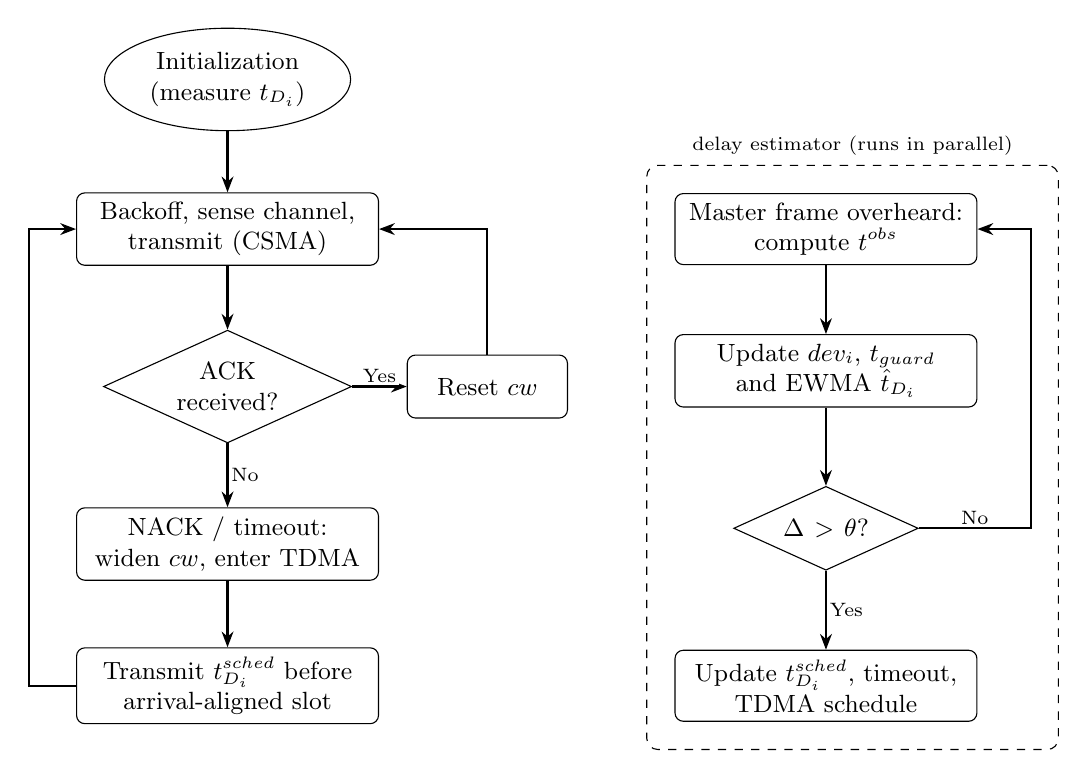
\begin{tikzpicture}[
    start/.style={ellipse, draw=black, fill=white, minimum width=2.3cm,
                  minimum height=0.9cm, align=center, font=\small},
    proc/.style={rectangle, draw=black, fill=white, text width=3.6cm,
                 minimum height=0.8cm, align=center, rounded corners=3pt, font=\small},
    dec/.style={diamond, draw=black, fill=white, text width=1.6cm,
                minimum height=0.7cm, align=center, font=\small, aspect=2.2, inner sep=1pt},
    arr/.style={-{Stealth[length=2mm]}, thick, draw=black},
    lbl/.style={font=\scriptsize, fill=white, inner sep=1pt}
]
% transmission logic (left)
\node[start] (init) at (0,0) {Initialization\\(measure $t_{D_i}$)};
\node[proc] (csma) at (0,-1.9) {Backoff, sense channel,\\transmit (CSMA)};
\node[dec]  (ack)  at (0,-3.9) {ACK\\received?};
\node[proc] (tdma) at (0,-5.9) {NACK / timeout:\\widen $cw$, enter TDMA};
\node[proc] (slot) at (0,-7.7) {Transmit $t^{sched}_{D_i}$ before\\arrival-aligned slot};
\node[proc, text width=1.8cm] (reset) at (3.3,-3.9) {Reset $cw$};
\draw[arr] (init) -- (csma);
\draw[arr] (csma) -- (ack);
\draw[arr] (ack) -- node[lbl, right]{No} (tdma);
\draw[arr] (ack) -- node[lbl, above]{Yes} (reset);
\draw[arr] (reset) |- (csma.east);
\draw[arr] (tdma) -- (slot);
\draw[arr] (slot.west) -- ++(-0.6,0) |- (csma.west);
% delay estimator (right, runs in parallel)
\node[proc] (obs)  at (7.6,-1.9) {Master frame overheard:\\compute $t^{obs}$};
\node[proc] (upd)  at (7.6,-3.7) {Update $dev_i$, $t_{guard}$\\and EWMA $\hat t_{D_i}$};
\node[dec]  (chg)  at (7.6,-5.7) {$\Delta > \theta$?};
\node[proc] (rec)  at (7.6,-7.7) {Update $t^{sched}_{D_i}$, timeout,\\TDMA schedule};
\coordinate (loop) at (10.2,-5.7);
\draw[arr] (obs) -- (upd);
\draw[arr] (upd) -- (chg);
\draw[arr] (chg) -- node[lbl, right]{Yes} (rec);
\draw[arr] (chg.east) -- node[lbl, above]{No} (loop) |- (obs.east);
\node[draw, dashed, rounded corners, inner sep=10pt, fit=(obs)(rec)(loop),
      label={[font=\scriptsize]above:delay estimator (runs in parallel)}] {};
\end{tikzpicture}
\caption{Flow of a sensor in Adaptive ARQ\_HMAC. The delay estimator (right) runs in parallel with the transmission logic (left) and changes the timeout and schedule it uses.}
\label{fig:adaptive_flowchart}
\end{figure}

\subsection{Justification of Design Choices} \label{sec:justification}
\begin{itemize}
    \item \textbf{EWMA with change detection.} The EWMA filter requires very little computation, just one multiplication and one addition per sample, and the threshold $\theta$ ensures that we do not break our schedule every time the estimate wobbles by an amount too small to actually cause a timing error.
    \item \textbf{Observations using overheard master frames.} Since ACKs and NACKs are already being sent regardless, we get delay observations essentially for free, with no extra frames on the wire. All we add is a 4-byte timestamp and a single byte for either the deviation or the destination address to frames that already exist.
    \item \textbf{Guard proportional to the measured variation, beginning with the value in the paper.} The design is safe from the start. The guard will only get smaller when the measured variation is truly tiny. In case the delay becomes unpredictable, $dev$ gets larger and the guard goes up again.
    \item \textbf{Arrival-aligned slots.} Aligning slots by when packets arrive rather than when they are transmitted strips $t_{max}$ out of the per-slot calculation entirely. This matters most in large networks where $t_{max}$ can easily exceed the packet transmission time.
    \item \textbf{Backoff with unit $2t_{max}$ and binary exponential window.} Setting the backoff unit to the maximum sensor-to-sensor propagation time means the randomization actually separates transmissions in a physically meaningful way. Doubling the window after errors lets the protocol adapt to whatever load the network is currently experiencing.
    \item \textbf{Standard, untuned constants.} The values of $\beta$, $K$, and the backoff rule come straight from RFC~6298 and IEEE~802.11, and the backoff unit is derived from the propagation physics. None of these were hand-tuned to our simulation results.
\end{itemize}

% ══════════════════════════════════════════════════════════
%  4. IMPLEMENTATION
% ══════════════════════════════════════════════════════════
\section{Implementation} \label{sec:implementation}

\subsection{Software Architecture in UnetStack}
We built both protocols on top of UnetStack~7.0~\cite{unetstack2014}, an agent-based protocol stack and discrete-event simulator for underwater networks, writing everything in Groovy. In UnetStack, each protocol lives inside an \emph{agent} that communicates with other agents on the same node by passing messages. Our MAC agent talks directly to the physical-layer agent (\texttt{phy}): it fires off \texttt{TxFrameReq} messages when it wants to transmit, and it listens for \texttt{RxFrameNtf} notifications when a frame has been decoded successfully or \texttt{BadFrameNtf} notifications when decoding fails, which the master treats as evidence of a collision. The simulator handles the acoustic propagation delay based on the actual positions of the nodes (including any that are moving) and drops frames that overlap at a receiver. The protocol code lives in \texttt{arqhmac/ArqHmacAgent.groovy}, the network scenario in \texttt{arqhmac/Scenario.groovy}, the experiment runner in \texttt{run\_comparison.groovy}, and the analysis scripts in \texttt{plot\_results.py}.

Rather than maintaining two separate codebases, we implemented both protocols inside a single agent class, \texttt{ArqHmacAgent}, controlled by a boolean flag called \texttt{proposed}. When \texttt{proposed = false}, the agent behaves exactly like the published ARQ\_HMAC. When \texttt{proposed = true}, it activates the five mechanisms from Section~\ref{sec:proposed_approach}. Keeping everything else identical means any performance gap we observe can be attributed squarely to the proposed mechanisms rather than to some unrelated implementation quirk. Figure~\ref{fig:classdiagram} lays out the class structure; the values in parentheses are the default parameters.

\begin{figure}[H]
\centering
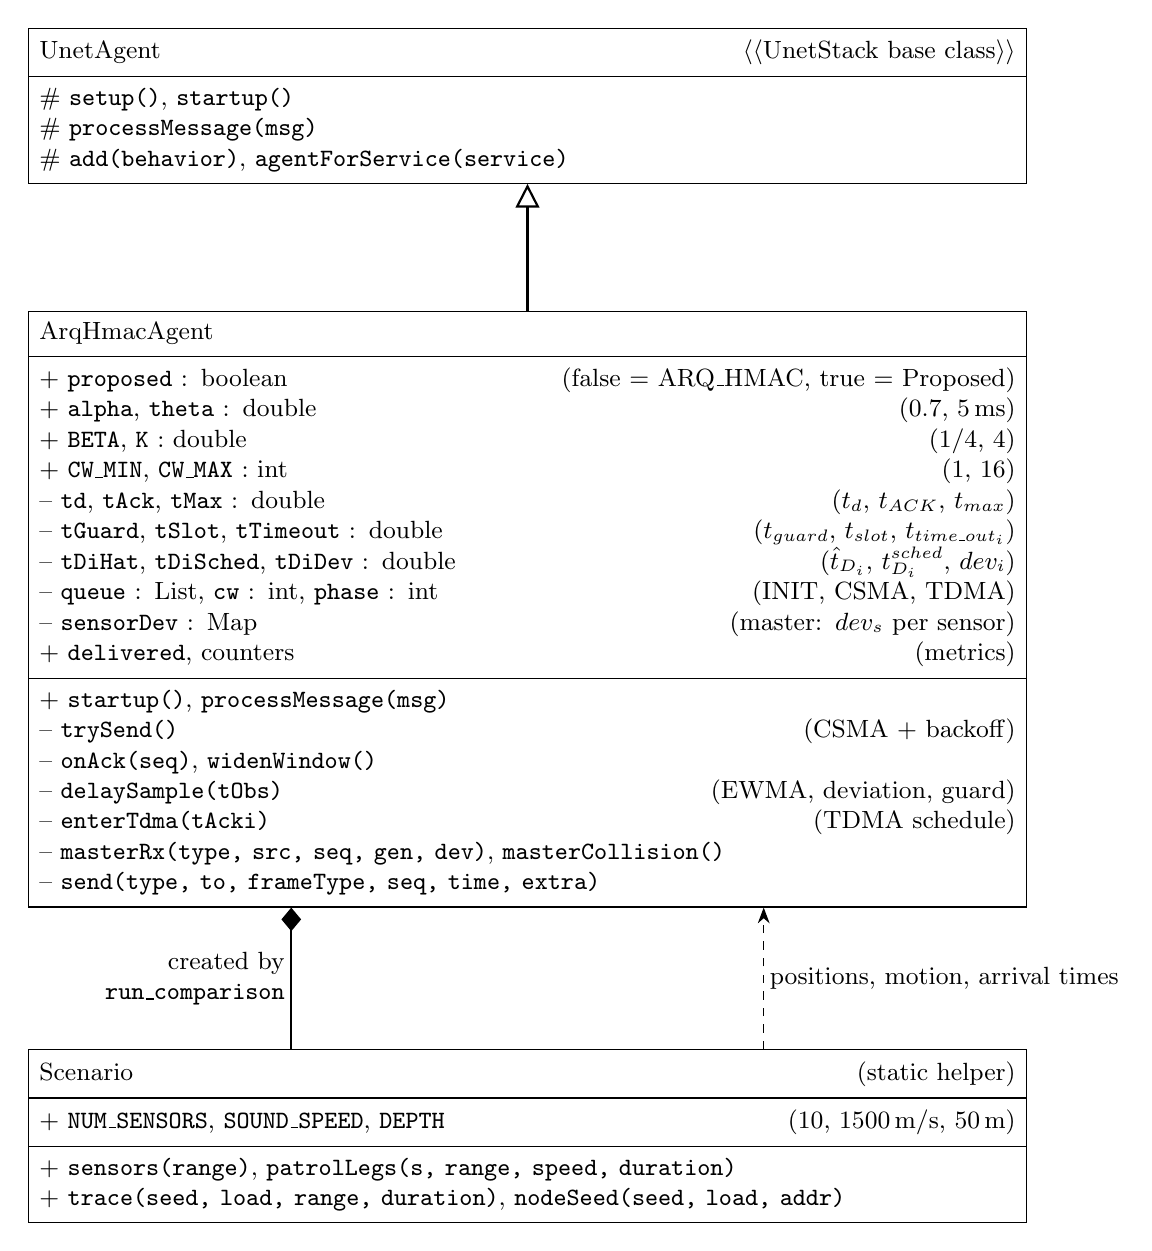
\begin{tikzpicture}[
    uml/.style={rectangle split, rectangle split parts=#1, draw=black, fill=white,
                font=\small, align=left, text width=12.4cm, inner sep=4pt},
    uml/.default=3,
    inh/.style={-{Triangle[open, length=3mm, width=3mm]}, thick},
    comp/.style={-{Diamond[length=3mm, width=2.5mm]}, thick},
    dep/.style={-{Stealth[length=2mm]}, dashed},
    lbl/.style={font=\small, fill=white, inner sep=2pt}
]
\node[uml=2] (unet) at (0,0) {
  UnetAgent \hfill $\langle\langle$UnetStack base class$\rangle\rangle$
  \nodepart{second}
  \# \texttt{setup()}, \texttt{startup()} \\
  \# \texttt{processMessage(msg)} \\
  \# \texttt{add(behavior)}, \texttt{agentForService(service)}
};
\node[uml, anchor=north] (agent) at (0,-2.6) {
  ArqHmacAgent
  \nodepart{second}
  + \texttt{proposed} : boolean \hfill (false = ARQ\_HMAC, true = Proposed)\\
  + \texttt{alpha}, \texttt{theta} : double \hfill (0.7, 5\,ms)\\
  + \texttt{BETA}, \texttt{K} : double \hfill (1/4, 4)\\
  + \texttt{CW\_MIN}, \texttt{CW\_MAX} : int \hfill (1, 16)\\
  -- \texttt{td}, \texttt{tAck}, \texttt{tMax} : double \hfill ($t_d$, $t_{ACK}$, $t_{max}$)\\
  -- \texttt{tGuard}, \texttt{tSlot}, \texttt{tTimeout} : double \hfill ($t_{guard}$, $t_{slot}$, $t_{time\_out_i}$)\\
  -- \texttt{tDiHat}, \texttt{tDiSched}, \texttt{tDiDev} : double \hfill ($\hat t_{D_i}$, $t^{sched}_{D_i}$, $dev_i$)\\
  -- \texttt{queue} : List, \texttt{cw} : int, \texttt{phase} : int \hfill (INIT, CSMA, TDMA)\\
  -- \texttt{sensorDev} : Map \hfill (master: $dev_s$ per sensor)\\
  + \texttt{delivered}, counters \hfill (metrics)
  \nodepart{third}
  + \texttt{startup()}, \texttt{processMessage(msg)}\\
  -- \texttt{trySend()} \hfill (CSMA + backoff)\\
  -- \texttt{onAck(seq)}, \texttt{widenWindow()}\\
  -- \texttt{delaySample(tObs)} \hfill (EWMA, deviation, guard)\\
  -- \texttt{enterTdma(tAcki)} \hfill (TDMA schedule)\\
  -- \texttt{masterRx(type, src, seq, gen, dev)}, \texttt{masterCollision()}\\
  -- \texttt{send(type, to, frameType, seq, time, extra)}
};
\node[uml, below=1.8cm of agent] (scen) {
  Scenario \hfill (static helper)
  \nodepart{second}
  + \texttt{NUM\_SENSORS}, \texttt{SOUND\_SPEED}, \texttt{DEPTH} \hfill (10, 1500\,m/s, 50\,m)
  \nodepart{third}
  + \texttt{sensors(range)}, \texttt{patrolLegs(s, range, speed, duration)}\\
  + \texttt{trace(seed, load, range, duration)}, \texttt{nodeSeed(seed, load, addr)}
};
\draw[inh] (agent.north) -- (unet.south);
\draw[comp] ($(scen.north)+(-3,0)$) -- node[lbl, left, align=right]{created by\\\texttt{run\_comparison}} ($(agent.south)+(-3,0)$);
\draw[dep] ($(scen.north)+(3,0)$) -- node[lbl, right]{positions, motion, arrival times} ($(agent.south)+(3,0)$);
\end{tikzpicture}
\caption{Class diagram of the implementation. Values in parentheses are the default parameters or the symbols used in Section~\ref{sec:proposed_approach}.}
\label{fig:classdiagram}
\end{figure}

\subsection{Key Subsystems}

\paragraph{Delay estimator.} The \texttt{delaySample(tObs)} routine carries out the calculations described in Eqs.~(\ref{eq:ewma}), (\ref{eq:deviation}) and (\ref{eq:guard}). It first tosses out any observation that looks physically impossible ($t^{obs} < 0$ or $t^{obs} > 2t_{max}$), then updates the deviation before touching the mean (following the RFC~6298 ordering), recomputes the guard and timeout, and only swaps in a new $t^{sched}_{D_i}$ when the shift exceeds $\theta$. This routine fires every time a sensor receives a master frame, regardless of who the frame was actually addressed to (see Algorithm~\ref{alg:delay}).

\paragraph{Backoff in \texttt{trySend()}.} The CSMA logic from ARQ\_HMAC stays the same, with one twist: a node that found the channel busy, or one that just exited a TDMA period, gets flagged as \emph{deferred} and has to wait a random interval before it can transmit. The contention window $cw$ gets adjusted whenever an ACK, NACK, or timeout occurs (Algorithm~\ref{alg:mods}).

\paragraph{Slots in \texttt{enterTdma()}.} The TDMA phase follows ARQ\_HMAC as well, except that the transmission timing and the end of the TDMA period now use the arrival-aligned slot formula from Eq.~(\ref{eq:aligned}), with whatever slot width the master announced (Algorithm~\ref{alg:mods}).

\paragraph{Master.} The master node runs ARQ\_HMAC with a few additions: it stamps its ACKs and NACKs with the transmission time, records the deviation value piggybacked on each incoming data packet, and picks a slot width large enough for the worst-case sensor before announcing it in the NACK (Algorithm~\ref{alg:mods}).

\paragraph{Frame format.} Every frame carries an 8-byte payload consisting of the frame type (INIT, DATA, ACK, NACK, or TDMA\_DATA), a 16-bit sequence number, a 32-bit time field in milliseconds, and one spare byte. In data frames the time field stores the packet's generation time (which we later use to compute end-to-end delay) and the extra byte holds the deviation $dev_i$. In master frames the time field carries the transmission start time for delay observations. ACKs use the extra byte for the destination address, while NACKs repurpose the sequence field to announce the TDMA slot width. The modem is set up so that a data frame takes $t_d = 1$~s to transmit and a control frame takes $t_{ACK} = 0.1$~s.

\subsection{Message Processing Path}
Figure~\ref{fig:processing} traces how \texttt{processMessage} handles each notification coming up from the physical layer; the step tagged [P] only exists in the proposed protocol. Algorithm~\ref{alg:delay} details the new delay estimator and Algorithm~\ref{alg:mods} lists the modifications to the existing ARQ\_HMAC handlers. The parts of the handlers that we did not change follow~\cite{dao2025} exactly and are not reproduced here.

\begin{algorithm}[H]
\caption{Delay observation (\texttt{delaySample}) [P]}
\label{alg:delay}
\begin{algorithmic}[1]
\REQUIRE observation $t^{obs}$
\ENSURE updated $\hat t_{D_i}$, $dev_i$, $t_{guard,i}$, $t^{sched}_{D_i}$, $t_{time\_out_i}$
\IF{$t^{obs} < 0$ \OR $t^{obs} > 2t_{max}$}
    \RETURN \COMMENTR{implausible sample}
\ENDIF
\STATE $dev_i \leftarrow (1-\beta)\,dev_i + \beta\,|t^{obs} - \hat t_{D_i}|$ \COMMENTR{deviation before mean}
\STATE $t_{guard,i} \leftarrow t_d + t_{ACK} + \max(t_{ACK}, 2K\,dev_i)$; \; $t_{time\_out_i} \leftarrow 2t^{sched}_{D_i} + t_{guard,i}$
\STATE $\hat t_{D_i} \leftarrow \alpha\, t^{obs} + (1-\alpha)\,\hat t_{D_i}$
\IF{$|\hat t_{D_i} - t^{sched}_{D_i}| > \theta$}
    \STATE $t^{sched}_{D_i} \leftarrow \hat t_{D_i}$; \; $t_{time\_out_i} \leftarrow 2t^{sched}_{D_i} + t_{guard,i}$
\ENDIF
\end{algorithmic}
\end{algorithm}

\begin{algorithm}[H]
\caption{Modifications to the ARQ\_HMAC handlers (only the changed lines)}
\label{alg:mods}
\begin{algorithmic}[1]
\STATE \textbf{trySend}, channel busy: deferred $\leftarrow$ true
\STATE \textbf{trySend}, channel free and deferred: deferred $\leftarrow$ false; wait $U(0,\, cw \cdot 2t_{max})$, then retry
\STATE \textbf{trySend}, sending DATA: add $dev_i$ to the frame; timer $\leftarrow 2t^{sched}_{D_i} + t_{guard,i}$
\STATE \textbf{onAck}: $cw \leftarrow 1$
\STATE \textbf{on timeout or NACK} for own packet: $cw \leftarrow \min(2cw, 16)$; on NACK $t_{slot} \leftarrow$ announced width
\STATE \textbf{enterTdma}: $t_{start} \leftarrow t_{ACK_i} + t_{max} - t^{sched}_{D_i}$; \; $t_{tx} \leftarrow t_{start} + t_{max} + n_i t_{slot} - t^{sched}_{D_i}$; \; $t_{end} \leftarrow t_{start} + t_{max} + n\,t_{slot}$
\STATE \textbf{end of TDMA}: deferred $\leftarrow$ true
\STATE \textbf{master, on DATA}: $dev_s \leftarrow$ reported deviation; ACK carries transmit time and destination
\STATE \textbf{master, on collision}: $t_{slot} \leftarrow t_d + t_{ACK} + \max(t_{ACK}, 2K \max_s dev_s)$; NACK carries $t_{slot}$ and transmit time
\end{algorithmic}
\end{algorithm}

\begin{figure}[H]
\centering
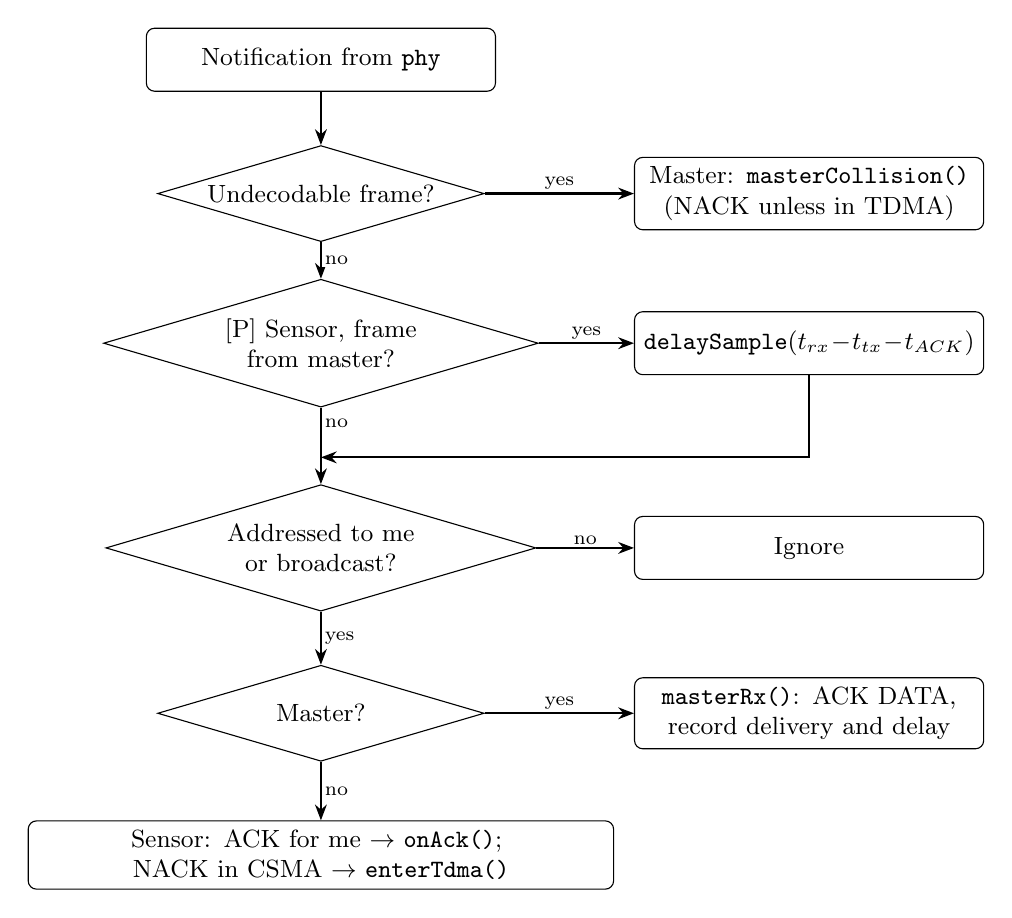
\begin{tikzpicture}[
    proc/.style={rectangle, draw=black, fill=white, text width=4.2cm,
                 minimum height=0.8cm, align=center, rounded corners=3pt, font=\small},
    dec/.style={diamond, draw=black, fill=white, text width=3.4cm,
                align=center, font=\small, aspect=3.4, inner sep=0pt},
    arr/.style={-{Stealth[length=2mm]}, thick, draw=black},
    lbl/.style={font=\scriptsize, fill=white, inner sep=1pt}
]
\node[proc] (in) at (0,0) {Notification from \texttt{phy}};
\node[dec]  (bad) at (0,-1.7) {Undecodable frame?};
\node[proc] (coll) at (6.2,-1.7) {Master: \texttt{masterCollision()}\\(NACK unless in TDMA)};
\node[dec]  (fromm) at (0,-3.6) {[P] Sensor, frame from master?};
\node[proc] (ds) at (6.2,-3.6) {\texttt{delaySample}($t_{rx} - t_{tx} - t_{ACK}$)};
\node[dec]  (forme) at (0,-6.2) {Addressed to me or broadcast?};
\node[proc] (drop) at (6.2,-6.2) {Ignore};
\node[dec]  (ism) at (0,-8.3) {Master?};
\node[proc] (mrx) at (6.2,-8.3) {\texttt{masterRx()}: ACK DATA,\\record delivery and delay};
\node[proc, text width=7.2cm] (srx) at (0,-10.1) {Sensor: ACK for me $\rightarrow$ \texttt{onAck()}; \; NACK in CSMA $\rightarrow$ \texttt{enterTdma()}};
\draw[arr] (in) -- (bad);
\draw[arr] (bad) -- node[lbl, above]{yes} (coll);
\draw[arr] (bad) -- node[lbl, right]{no} (fromm);
\draw[arr] (fromm) -- node[lbl, above]{yes} (ds);
\coordinate (join) at ($(fromm.south)!0.65!(forme.north)$);
\draw[arr] (fromm) -- node[lbl, right, pos=0.2]{no} (forme);
\draw[arr] (ds.south) |- (join);
\draw[arr] (forme) -- node[lbl, above]{no} (drop);
\draw[arr] (forme) -- node[lbl, right]{yes} (ism);
\draw[arr] (ism) -- node[lbl, above]{yes} (mrx);
\draw[arr] (ism) -- node[lbl, right]{no} (srx);
\end{tikzpicture}
\caption{Flow of \texttt{processMessage} for every notification from the physical layer.}
\label{fig:processing}
\end{figure}

\subsection{Complexity and Overhead}
\begin{itemize}
    \item \textbf{Computations.} Each delay observation boils down to a handful of $O(1)$ arithmetic operations. The master has to find the maximum deviation across all reported DATA packets once per NACK, which takes $O(n)$ operations for $n$ sensors, hardly a bottleneck.
    \item \textbf{Memory.} A sensor needs to stash five extra numbers ($\hat t_{D_i}$, $t^{sched}_{D_i}$, $dev_i$, $t_{guard,i}$, $cw$). The master keeps one deviation value per sensor. The footprint is negligible.
    \item \textbf{Communication.} We did not introduce any new frame types. The timestamp and the extra byte squeeze into the existing 8-byte payload, so control frames stay at their original duration of $t_{ACK} = 0.1$~s.
\end{itemize}

\subsection{Configurable Parameters}
The values of the protocol parameters are outlined in Table~\ref{tab:protoparams}. These were finalized prior to experimentation on the basis of existing standards and fundamental considerations. The different tuning seeds (101--105) were utilized for determining the inclusion/exclusion of certain mechanisms in general, and not individual parameters.

\begin{table}[H]
\centering
\caption{Protocol parameters used in the experiments.}
\label{tab:protoparams}
\small
\setstretch{1.1}
\begin{tabular}{@{}llc@{}}
\toprule
\textbf{Parameter} & \textbf{Meaning} & \textbf{Value} \\
\midrule
$\alpha$ & EWMA smoothing factor & 0.7 \\
$\theta$ & Change-detection threshold & 5 ms \\
$\beta$, $K$ & Deviation gain, guard multiplier (RFC 6298) & 1/4, 4 \\
$dev_i^{(0)}$ & Initial deviation & $t_d/(2K)$ \\
$t_{guard}$ & Guard (baseline / proposed) & $2t_d + t_{ACK}$ / Eq.~(\ref{eq:guard}) \\
$cw$ & Contention window, unit $2t_{max}$ & 1 \ldots\ 16 \\
-- & Carrier re-check interval & 10 ms \\
\bottomrule
\end{tabular}
\end{table}

\paragraph{Deviations from the paper.} The original paper defines the slot index as $n_i = \lfloor t_{D_i} / t_{slot} \rfloor$. Since $t_{D_i} < t_{max} < t_{slot}$ in practice, this expression always evaluates to zero, which would dump every node into the same slot. Both of our implementations sidestep this by assigning each sensor its own slot based on its index in the network, which is consistent with the TDMA period of $n\,t_{slot}$. We also broadcast ACKs with the destination embedded in the payload in both protocol variants; this does not alter ARQ\_HMAC's behaviour in any meaningful way. While implementing this solution, we tried out another mechanism which was a block acknowledgment for TDMA retransmissions on the tuning seeds; this was effective only at light loads and led to congestion collapse during heavy loads, hence we abandoned it.
% ══════════════════════════════════════════════════════════
%  5. RESULTS AND ANALYSIS
% ══════════════════════════════════════════════════════════
\section{Results and Analysis} \label{sec:results}

\subsection{Simulation Setup}
We ran both protocols in UnetStack~7.0 using the \texttt{ProtocolChannelModel}. The master node sits moored in the middle of the deployment area. Around it are four moored sensors at distances between $0.38R$ and $0.75R$, plus six AUV sensors. Each AUV moves back and forth along a radial path between $0.2R$ and $0.85R$, with its own bearing and starting position, so its delay to the master is always changing. Every sensor can reach the master, but sensors on opposite sides cannot hear one another, which produces hidden terminals much like those in a real deployment. We consider three channel conditions (Table~\ref{tab:scenarios}); the remaining parameters appear in Table~\ref{tab:params}. For each combination of condition, load and seed we generate a single traffic trace and feed it to both protocols. The script also verifies that the two protocols produced exactly the same set of packets.

\begin{table}[H]
\centering
\caption{Channel conditions.}
\label{tab:scenarios}
\small
\setstretch{1.1}
\begin{tabular}{@{}llll@{}}
\toprule
\textbf{Condition} & \textbf{Range $R$} & \textbf{AUV speed} & \textbf{One-way delay change} \\
\midrule
Static-400m & 400 m & 0 (all fixed, paper setup) & none \\
Mobile-400m & 400 m & 0.3 m/s & up to 0.17 s \\
Mobile-3km & 3000 m & 2 m/s & up to 1.3 s \\
\bottomrule
\end{tabular}
\end{table}

\begin{table}[H]
\centering
\caption{Simulation parameters.}
\label{tab:params}
\small
\setstretch{1.1}
\begin{tabular}{@{}ll@{}}
\toprule
\textbf{Parameter} & \textbf{Value} \\
\midrule
Simulator & UnetStack 7.0, \texttt{ProtocolChannelModel} \\
Nodes & 1 master + 10 sensors (4 moored, 6 AUVs), depth 50 m \\
Sound speed & 1500 m/s \\
Data rate & 1200 bps \\
Data / control packet & 1200 bits ($t_d = 1$ s) / 120 bits ($t_{ACK} = 0.1$ s) \\
Communication range $R$ & 400 m ($t_{max} = 0.27$ s) or 3000 m ($t_{max} = 2$ s) \\
Traffic & Poisson, offered load $G \in \{0.05, 0.1, 0.2, 0.3\}$ \\
Duration & 1800 s per run \\
Repetitions & 10 seeds per (condition, load), 240 runs in total \\
Compared protocols & ARQ\_HMAC, Adaptive ARQ\_HMAC \\
\bottomrule
\end{tabular}
\end{table}

We define the offered load $G$ as the number of newly generated packets per data-packet duration across the entire network. For example, $G = 0.1$ corresponds to one new packet every 10 seconds, shared among the ten sensors. The modem settings are taken from Table~2 of the ARQ\_HMAC paper~\cite{dao2025}.

\subsection{Performance Metrics}
\begin{itemize}
    \item \textbf{Packet Delivery Ratio (PDR)}: the number of distinct packets that reached the master, divided by the number generated.
    \item \textbf{Throughput $S$}: delivered packets multiplied by $t_d$ and divided by the operating time. This is the share of time the channel spends carrying successful data, following the definition in the paper.
    \item \textbf{Number of retransmissions}: packets that were resent in a TDMA slot after their CSMA attempt failed.
    \item \textbf{Collision rate}: collisions detected at the master divided by the frames the sensors sent.
    \item \textbf{End-to-end delay}: the time between a packet being generated and its first reception at the master.
    \item \textbf{Delay estimate error} (diagnostic): the mean absolute gap between the delay value a sensor is using and its true delay derived from its position, sampled every 10~s.
\end{itemize}
Since both protocols receive identical traffic, we compare their runs pairwise using the two-sided Wilcoxon signed-rank test (40 pairs per condition). A difference counts as significant when $p < 0.05$.

\subsection{Numerical Results}
Table~\ref{tab:summary} gives the outcome of all 240 simulations, averaged over the four loads and ten seeds. The proposed protocol is better on every metric in every condition, and each difference is statistically significant ($p < 0.001$). The ``B/E/W'' column gives the number of paired runs in which the proposed protocol was better, equal or worse than ARQ\_HMAC. Table~\ref{tab:perload} splits the results by offered load.

\begin{table}[H]
\centering
\caption{Overall results (mean over 4 loads $\times$ 10 seeds; all $p < 0.001$).}
\label{tab:summary}
\small
\setstretch{1.1}
\begin{tabular}{@{}llrrrr@{}}
\toprule
\textbf{Condition} & \textbf{Metric} & \textbf{ARQ\_HMAC} & \textbf{Proposed} & \textbf{Change} & \textbf{B/E/W} \\
\midrule
\multirow{5}{*}{Static-400m} & PDR (\%) & 93.08 & \textbf{96.30} & +3.5\% & 22/13/5 \\
 & Throughput $S$ & 0.144 & \textbf{0.153} & +6.5\% & 22/13/5 \\
 & Retransmissions & 138.1 & \textbf{75.9} & $-$45.1\% & 36/4/0 \\
 & Collision rate (\%) & 10.37 & \textbf{7.92} & $-$23.6\% & 27/3/10 \\
 & End-to-end delay (s) & 12.01 & \textbf{3.96} & $-$67.0\% & 39/0/1 \\
\midrule
\multirow{5}{*}{Mobile-400m} & PDR (\%) & 92.72 & \textbf{95.92} & +3.4\% & 22/10/8 \\
 & Throughput $S$ & 0.143 & \textbf{0.152} & +6.3\% & 22/10/8 \\
 & Retransmissions & 134.2 & \textbf{75.4} & $-$43.8\% & 36/3/1 \\
 & Collision rate (\%) & 10.42 & \textbf{8.06} & $-$22.7\% & 27/2/11 \\
 & End-to-end delay (s) & 11.26 & \textbf{3.93} & $-$65.1\% & 39/0/1 \\
\midrule
\multirow{5}{*}{Mobile-3km} & PDR (\%) & 79.46 & \textbf{89.34} & +12.4\% & 30/8/2 \\
 & Throughput $S$ & 0.110 & \textbf{0.135} & +22.7\% & 30/8/2 \\
 & Retransmissions & 176.9 & \textbf{94.3} & $-$46.7\% & 40/0/0 \\
 & Collision rate (\%) & 17.42 & \textbf{12.22} & $-$29.9\% & 39/1/0 \\
 & End-to-end delay (s) & 89.37 & \textbf{25.11} & $-$71.9\% & 40/0/0 \\
\bottomrule
\end{tabular}
\end{table}

\begin{table}[H]
\centering
\caption{Results per offered load (ARQ\_HMAC $\rightarrow$ Proposed, mean over 10 seeds).}
\label{tab:perload}
\small
\setstretch{1.1}
\resizebox{\textwidth}{!}{%
\begin{tabular}{@{}llccccc@{}}
\toprule
\textbf{Condition} & $G$ & \textbf{PDR (\%)} & \textbf{Throughput $S$} & \textbf{Retransmissions} & \textbf{Collisions (\%)} & \textbf{Delay (s)} \\
\midrule
\multirow{4}{*}{Static-400m} & 0.05 & 99.8 $\rightarrow$ 99.9 & 0.050 $\rightarrow$ 0.050 & 6.7 $\rightarrow$ 4.2 & 2.0 $\rightarrow$ 1.9 & 2.0 $\rightarrow$ 1.7 \\
 & 0.10 & 99.2 $\rightarrow$ 99.4 & 0.098 $\rightarrow$ 0.098 & 27.0 $\rightarrow$ 19.9 & 4.7 $\rightarrow$ 4.2 & 3.5 $\rightarrow$ 2.4 \\
 & 0.20 & 94.2 $\rightarrow$ 95.9 & 0.188 $\rightarrow$ 0.191 & 153.3 $\rightarrow$ 86.2 & 13.2 $\rightarrow$ 10.2 & 12.3 $\rightarrow$ 4.4 \\
 & 0.30 & 79.1 $\rightarrow$ 90.0 & 0.241 $\rightarrow$ 0.275 & 365.5 $\rightarrow$ 193.2 & 21.5 $\rightarrow$ 15.3 & 30.3 $\rightarrow$ 7.4 \\
\midrule
\multirow{4}{*}{Mobile-400m} & 0.05 & 99.9 $\rightarrow$ 100.0 & 0.050 $\rightarrow$ 0.050 & 6.5 $\rightarrow$ 4.4 & 1.7 $\rightarrow$ 1.7 & 2.0 $\rightarrow$ 1.7 \\
 & 0.10 & 99.1 $\rightarrow$ 98.7 & 0.098 $\rightarrow$ 0.097 & 27.0 $\rightarrow$ 18.3 & 4.9 $\rightarrow$ 4.6 & 3.5 $\rightarrow$ 2.2 \\
 & 0.20 & 93.1 $\rightarrow$ 96.5 & 0.185 $\rightarrow$ 0.192 & 149.0 $\rightarrow$ 80.9 & 13.2 $\rightarrow$ 9.5 & 11.8 $\rightarrow$ 4.2 \\
 & 0.30 & 78.8 $\rightarrow$ 88.4 & 0.240 $\rightarrow$ 0.270 & 354.4 $\rightarrow$ 198.0 & 21.9 $\rightarrow$ 16.4 & 27.7 $\rightarrow$ 7.5 \\
\midrule
\multirow{4}{*}{Mobile-3km} & 0.05 & 99.7 $\rightarrow$ 100.0 & 0.050 $\rightarrow$ 0.050 & 23.1 $\rightarrow$ 9.2 & 6.0 $\rightarrow$ 3.3 & 8.0 $\rightarrow$ 4.1 \\
 & 0.10 & 95.5 $\rightarrow$ 97.3 & 0.094 $\rightarrow$ 0.096 & 79.3 $\rightarrow$ 37.0 & 12.7 $\rightarrow$ 8.3 & 20.4 $\rightarrow$ 7.0 \\
 & 0.20 & 72.6 $\rightarrow$ 88.3 & 0.144 $\rightarrow$ 0.176 & 260.0 $\rightarrow$ 131.8 & 23.7 $\rightarrow$ 15.9 & 91.9 $\rightarrow$ 18.6 \\
 & 0.30 & 50.0 $\rightarrow$ 71.8 & 0.152 $\rightarrow$ 0.219 & 345.2 $\rightarrow$ 199.2 & 27.3 $\rightarrow$ 21.4 & 237.2 $\rightarrow$ 70.7 \\
\bottomrule
\end{tabular}%
}
\end{table}

\subsection{Graphical Analysis}

\paragraph{Delay tracking.} Figure~\ref{fig:tracking} illustrates the main idea of the proposal for a single AUV over one complete run. The true delay of this vehicle varies between 55~ms and 225~ms. ARQ\_HMAC stays with the 135~ms value it measured at start-up and is therefore off by as much as 90~ms, whereas the proposed protocol stays within a few milliseconds of the real value. Averaged over all sensors, the delay estimate error drops from 36.3~ms to 3.0~ms in Mobile-400m and from 306~ms to 15~ms in Mobile-3km, which is a reduction of 92\% and 95\% respectively. In the static network both protocols measure the delay only once, so their estimates are the same.

\begin{figure}[H]
\centering
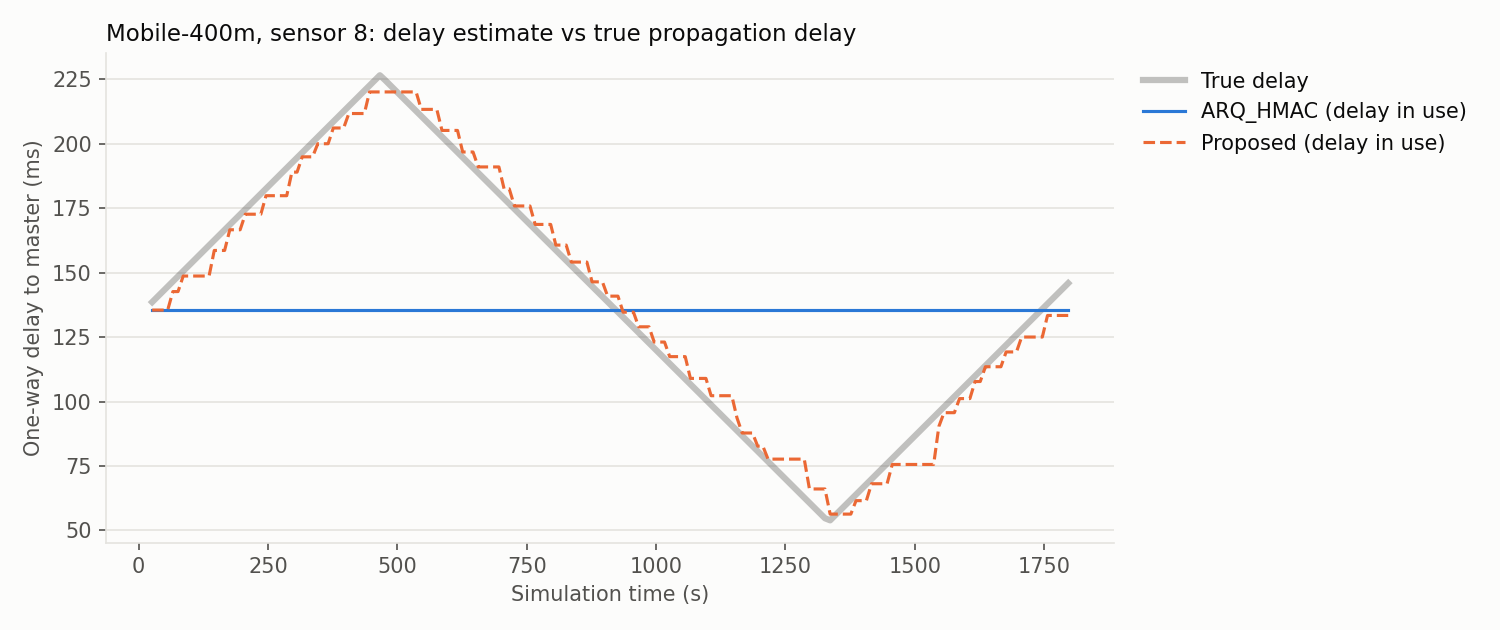
\includegraphics[width=\textwidth]{fig_estimate_tracking.png}
\caption{Delay value in use versus true propagation delay of one AUV (Mobile-400m, $G = 0.1$). ARQ\_HMAC keeps its start-up measurement; the proposed protocol follows the moving AUV.}
\label{fig:tracking}
\end{figure}

\paragraph{End-to-end delay.} End-to-end delay improves the most dramatically by reducing the end-to-end delay in 65--72\% under all conditions (see Figures~\ref{fig:static}--\ref{fig:mobile3km}). When the guard is correctly estimated, it may be reduced from 2.1~s to roughly 1.2--1.4~s, and the arrival-aligned slots take $t_{max}$ out of each slot. As a result, a TDMA period for ten sensors lasts 12--16~s, compared with 24~s at 400~m and 41~s at 3~km for the baseline. Retransmitted packets get to the master earlier, and the channel goes back to CSMA sooner. The improvement grows with load, since a larger share of packets passes through TDMA periods and queues start to build.

\begin{figure}[H]
\centering
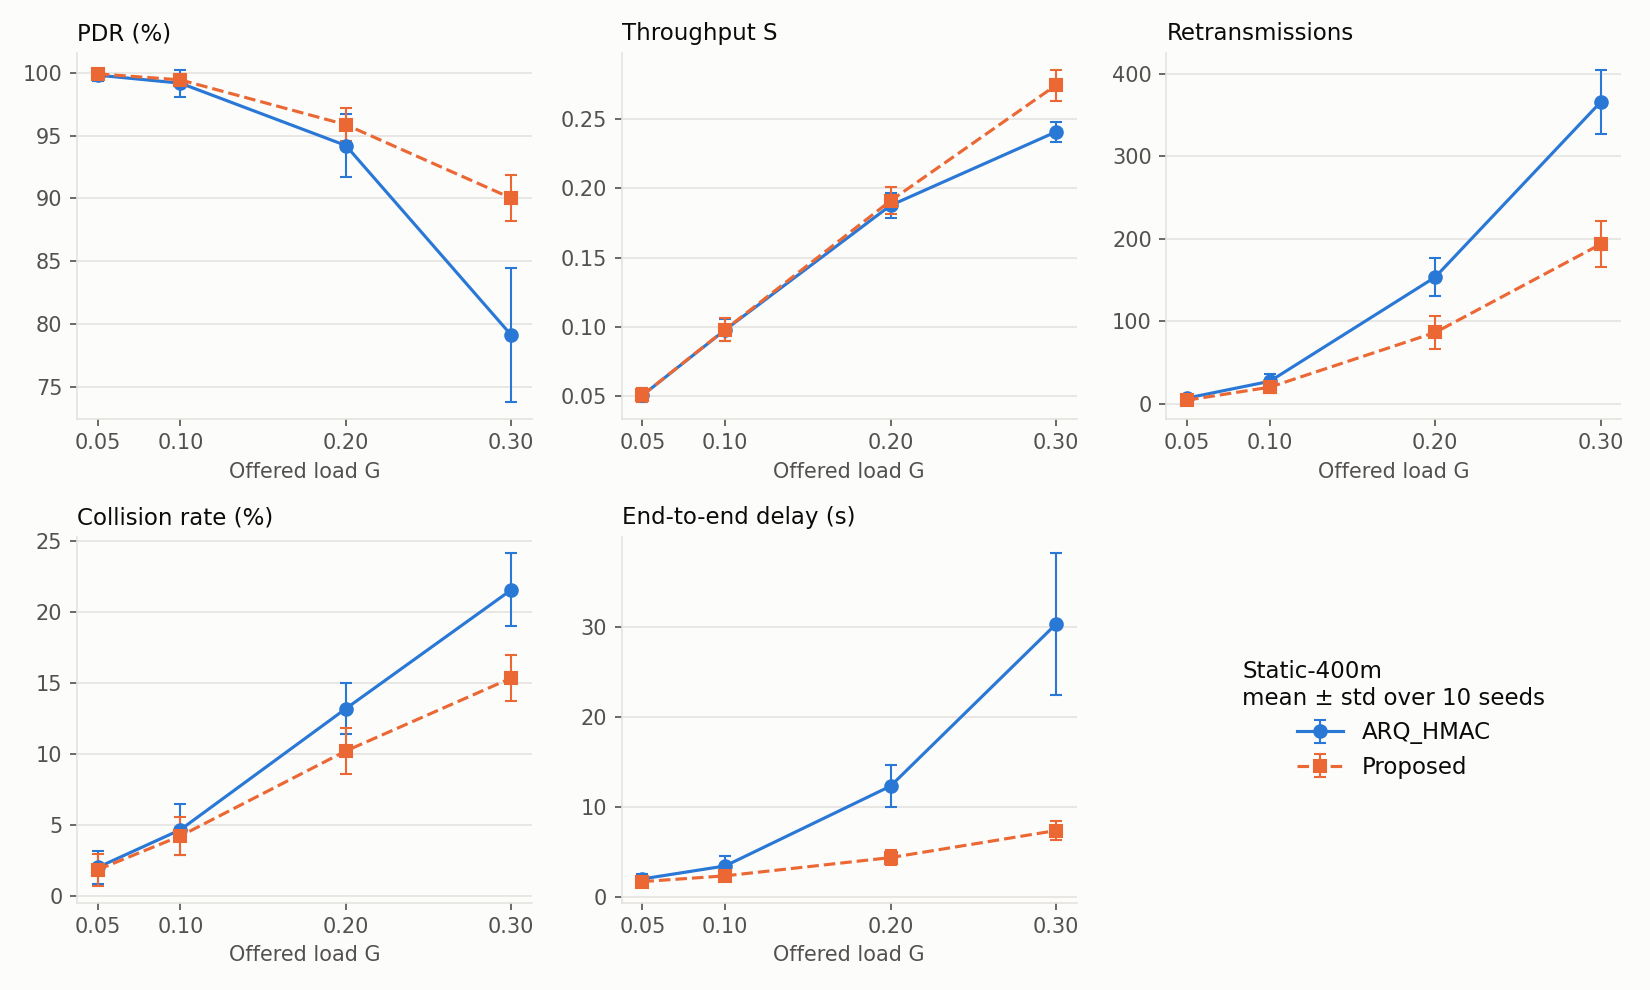
\includegraphics[width=\textwidth]{fig_Static-400m.png}
\caption{Static-400m: PDR, throughput, retransmissions, collision rate and end-to-end delay versus offered load.}
\label{fig:static}
\end{figure}

\paragraph{Retransmissions and collisions.} The number of retransmissions goes down by 44--47\% and the collision rate by 23--30\%. Adaptive backoff desynchronises nodes that finish a TDMA period at the same moment or that wait on the same busy channel. This eliminates many of the collisions that would otherwise trigger another TDMA period. In addition, the shorter timeouts let a node notice a lost packet sooner.

\begin{figure}[H]
\centering
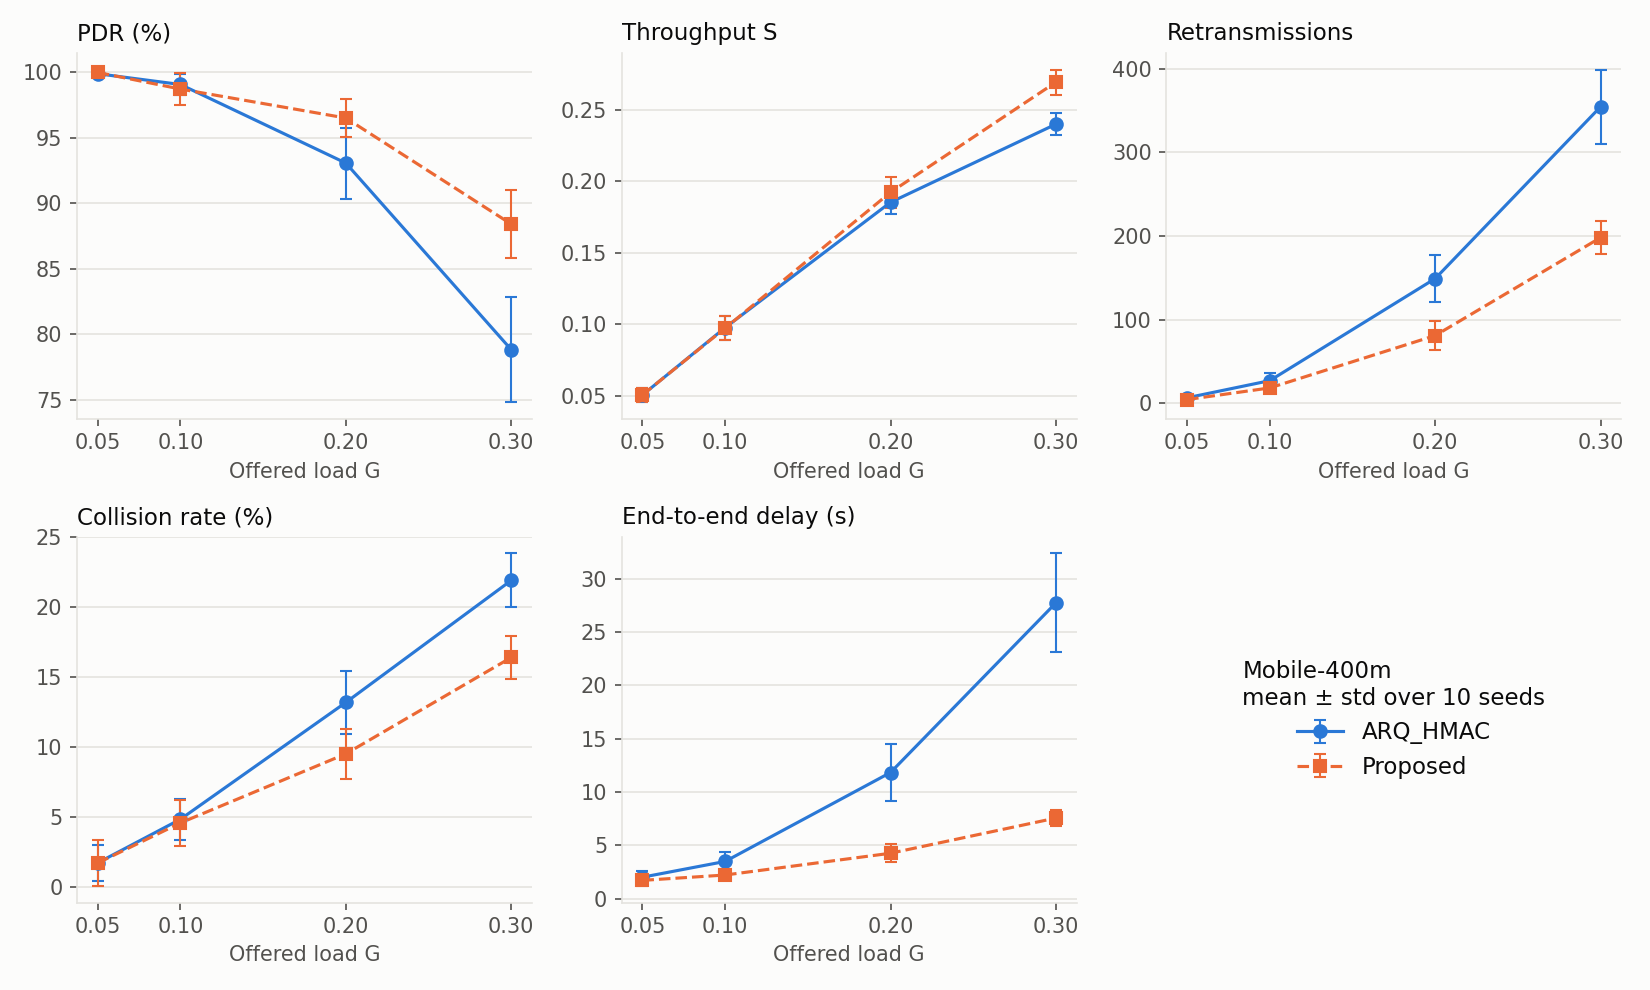
\includegraphics[width=\textwidth]{fig_Mobile-400m.png}
\caption{Mobile-400m: PDR, throughput, retransmissions, collision rate and end-to-end delay versus offered load.}
\label{fig:mobile400}
\end{figure}

\paragraph{PDR and throughput.} When the load is light, the channel is seldom contended and both protocols deliver nearly everything. At high load, the long TDMA periods and frequent collisions of the baseline lead to losses, and at $G = 0.3$ its PDR falls to 79\% at 400~m and 50\% at 3~km. The proposed protocol holds PDR at 88--90\% at 400~m and 72\% at 3~km, and its throughput continues to climb with load while the baseline levels off (Figure~\ref{fig:mobile3km}). The 3~km network gains the most (+22.7\% throughput, +12.4\% PDR), since $t_{max}$ is largest there and so a precise delay value matters most.

\begin{figure}[H]
\centering
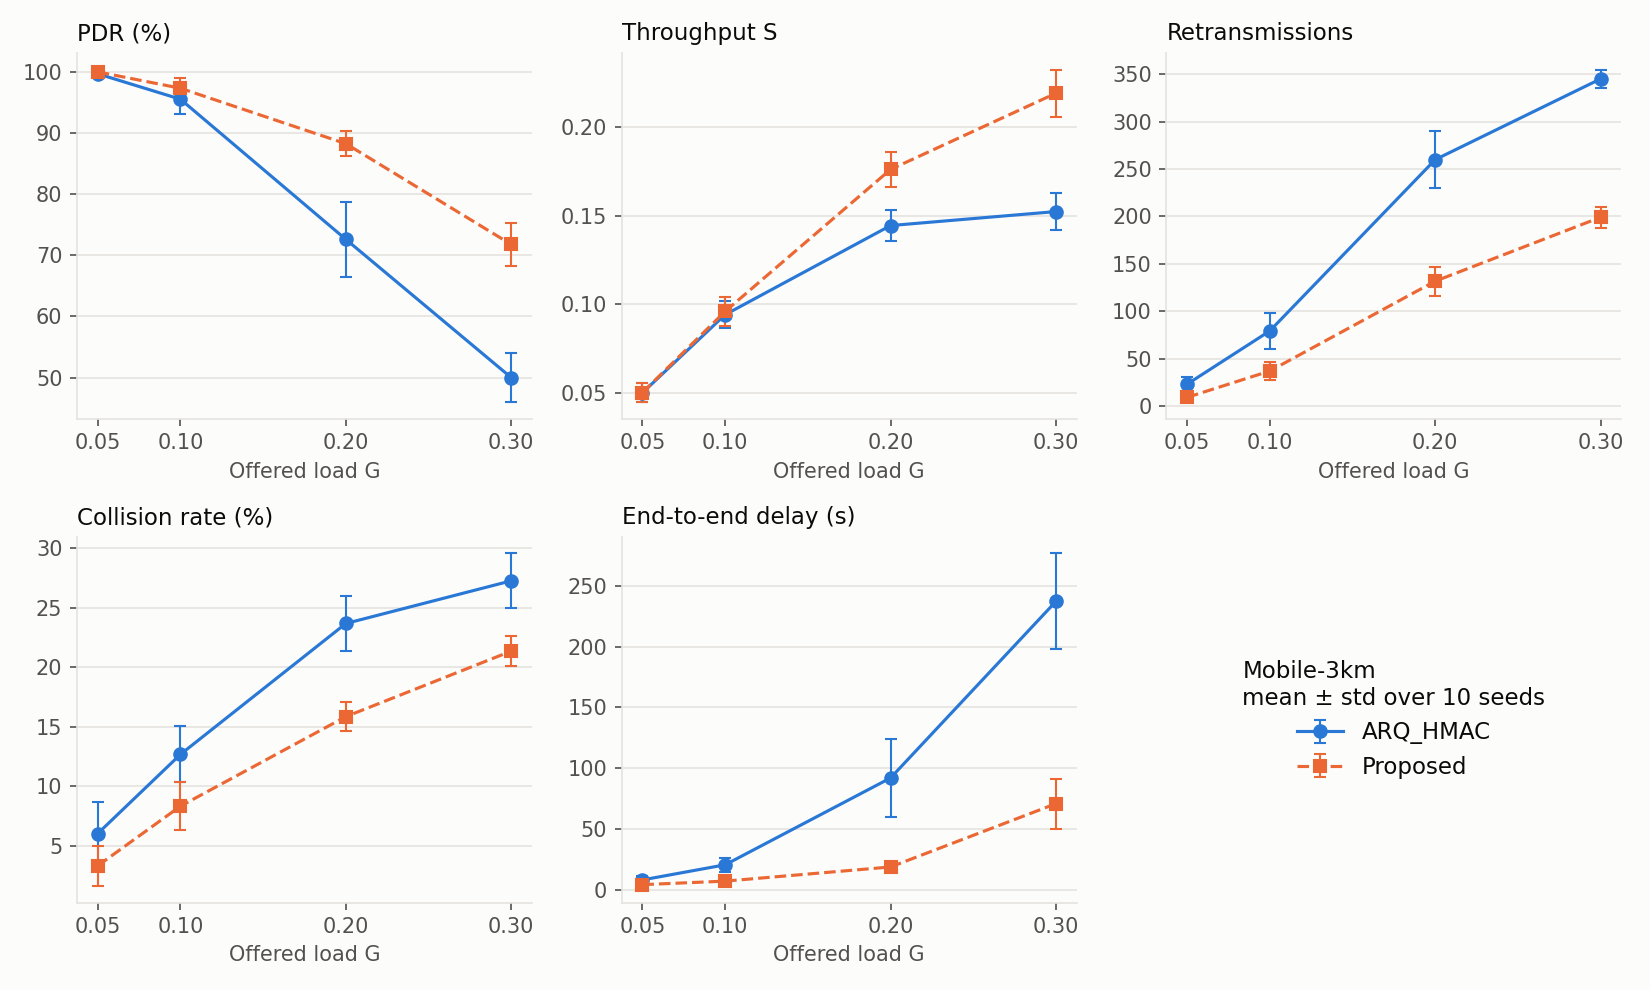
\includegraphics[width=\textwidth]{fig_Mobile-3km.png}
\caption{Mobile-3km: PDR, throughput, retransmissions, collision rate and end-to-end delay versus offered load.}
\label{fig:mobile3km}
\end{figure}

\paragraph{Static network.} The proposed protocol is significantly better even when no node moves. The measured delay variation is small, so the adaptive guard and aligned slots can shorten the timing without risk. The gain is therefore not only a result of mobility: the fixed margins in the paper are conservative, and tracking the delay continuously makes it possible to trim them.

\subsection{Comparison with the State of the Art}
Among hybrid ARQ-based MAC protocols for UASNs, ARQ\_HMAC is the most recent, and its authors reported higher and steadier throughput than Pure ALOHA, ALOHA with CSMA, Slotted ALOHA and Slotted ALOHA with CSMA~\cite{dao2025}. Table~\ref{tab:sota} compares the reviewed schemes at the design level, and the bullets below connect those design differences to our measurements.

\begin{table}[H]
\centering
\caption{Design level comparison with the state of the art.}
\label{tab:sota}
\small
\setstretch{1.1}
\begin{tabular}{@{}lccccc@{}}
\toprule
\textbf{Protocol} & \textbf{\shortstack{Collision-free\\retransmission}} & \textbf{\shortstack{Delay\\aware}} & \textbf{\shortstack{Continuous\\delay update}} & \textbf{\shortstack{Adaptive\\timing margin}} & \textbf{\shortstack{Adaptive\\contention}} \\
\midrule
Slotted FAMA~\cite{slottedfama2006} & No & No & No & No & No \\
T-Lohi~\cite{tlohi2008} & No & No & No & No & Yes \\
DOTS~\cite{dots2014} & No & Yes & Yes & No & No \\
Asym-TDMA~\cite{cho2018} & Yes & Yes & Periodic & No & No \\
ARQ\_HMAC~\cite{dao2025} & Yes & Yes & No & No & No \\
\textbf{Adaptive ARQ\_HMAC} & \textbf{Yes} & \textbf{Yes} & \textbf{Yes} & \textbf{Yes} & \textbf{Yes} \\
\bottomrule
\end{tabular}
\end{table}

\begin{itemize}
    \item \textbf{Versus ARQ\_HMAC.} With identical traffic and node motion, the proposed protocol gives a significant improvement on all five metrics in the static network, in the mobile network of the size used in the paper, and in the long-range mobile network. Delay is 65--72\% lower, retransmissions are 44--47\% fewer, collisions are 23--30\% fewer, throughput is 6--23\% higher and PDR is 3--12\% higher.
    \item \textbf{Versus the protocols ARQ\_HMAC was compared with.} In the paper's evaluation ARQ\_HMAC beats the ALOHA and CSMA variants, and here the proposed protocol beats ARQ\_HMAC. We therefore expect it to beat those variants too, but we did not simulate them again.
    \item \textbf{Versus delay-aware protocols.} Like DOTS, the proposed protocol learns delays from overheard, timestamped traffic. It differs by keeping the collision-free retransmission phase of ARQ\_HMAC and using the delay knowledge to make that phase shorter. Compared with Asym-TDMA, it updates the delay continuously rather than at fixed intervals. These comparisons rest on design alone, because DOTS and Asym-TDMA were not simulated.
\end{itemize}

\subsection{Discussion and Limitations}
The experiments show that continuous delay tracking combined with adaptive timing improves ARQ\_HMAC under every condition we tested, most clearly in the large network and at heavy load. At light load ($G \le 0.1$) the differences in PDR and throughput stay within $\pm 2\%$, and in one case (Mobile-400m, $G = 0.1$) PDR is marginally lower (98.7\% versus 99.1\%). As in the paper, TDMA retransmissions are not acknowledged, so a frame lost in a slot stays lost in both protocols. The timestamped observations rely on synchronised clocks. These are perfect in the simulator, but a real deployment would need periodic resynchronisation. Lastly, the protocol channel model has no bit errors, multipath or sound-speed variation, so all delay changes in the simulation come from node motion alone.

% ══════════════════════════════════════════════════════════
%  6. CONCLUSION
% ══════════════════════════════════════════════════════════
\section{Conclusions and Future Work} \label{sec:conclusion}

This work set out to remove a major weakness of ARQ\_HMAC. Its retransmission scheduling depends on a propagation delay that is measured once at start-up and then covered by large fixed timing margins, even though underwater delays change with conditions and node movement. We proposed Adaptive ARQ\_HMAC, which refreshes the delay estimate continuously with an EWMA filter and change detection, takes observations from timestamped master frames, derives its guard time from the measured delay variation, aligns TDMA slots with packet arrivals, and adjusts its backoff to the level of contention.

We implemented both protocols in UnetStack and compared them on identical traffic in 240 simulations. The proposed protocol follows the true delay with a mean error of 3~ms at 400~m and 15~ms at 3~km. Across the static, mobile and long-range scenarios it lowers end-to-end delay by 65--72\%, retransmissions by 44--47\% and collisions by 23--30\%, and it raises throughput by 6--23\% and packet delivery ratio by 3--12\%. All of these differences are statistically significant.

Future work includes a stable acknowledgement scheme for TDMA retransmissions and clock-drift compensation for the timestamped observations. It also includes more realistic channel models with bit errors, multipath and sound-speed variation, energy measurements, and tests on real acoustic modems.

% ══════════════════════════════════════════════════════════
%  REFERENCES
% ══════════════════════════════════════════════════════════
\begin{thebibliography}{00}

\bibitem{dao2025}
V.-P. Dao and T.-H. Tran,
``ARQ\_HMAC: An automatic repeat request strategy for hybrid MAC protocol in underwater acoustic sensor networks,''
\textit{IEEE Access}, vol. 13, pp. 159196--159206, 2025, doi: \href{https://doi.org/10.1109/ACCESS.2025.3607746}{10.1109/ACCESS.2025.3607746}.

\bibitem{akyildiz2005}
I. F. Akyildiz, D. Pompili and T. Melodia,
``Underwater acoustic sensor networks: Research challenges,''
\textit{Ad Hoc Networks}, vol. 3, no. 3, pp. 257--279, 2005, doi: \href{https://doi.org/10.1016/j.adhoc.2005.01.004}{10.1016/j.adhoc.2005.01.004}.

\bibitem{casari2011}
P. Casari and M. Zorzi,
``Protocol design issues in underwater acoustic networks,''
\textit{Computer Communications}, vol. 34, no. 17, pp. 2013--2025, 2011, doi: \href{https://doi.org/10.1016/j.comcom.2011.06.008}{10.1016/j.comcom.2011.06.008}.

\bibitem{jiang2018}
S. Jiang,
``State-of-the-art medium access control (MAC) protocols for underwater acoustic networks: A survey based on a MAC reference model,''
\textit{IEEE Communications Surveys \& Tutorials}, vol. 20, no. 1, pp. 96--131, 2018, doi: \href{https://doi.org/10.1109/COMST.2017.2768802}{10.1109/COMST.2017.2768802}.

\bibitem{kulla2022}
E. Kulla, K. Matsuo and L. Barolli,
``MAC layer protocols for underwater acoustic sensor networks: A survey,''
\textit{Lecture Notes in Networks and Systems}, vol. 496, pp. 211--220, 2022, doi: \href{https://doi.org/10.1007/978-3-031-08819-3_21}{10.1007/978-3-031-08819-3\_21}.

\bibitem{cho2018}
A.-R. Cho, C. Yun, Y.-K. Lim and Y. Choi,
``Asymmetric propagation delay-aware TDMA MAC protocol for mobile underwater acoustic sensor networks,''
\textit{Applied Sciences}, vol. 8, no. 6, p. 962, 2018, doi: \href{https://doi.org/10.3390/app8060962}{10.3390/app8060962}.

\bibitem{molinares2009}
D. J. Molinares and M. A. Labrador,
``An adaptive logical link layer protocol for underwater acoustic communication channels,''
in \textit{Proc. OCEANS 2009}, 2009, pp. 1--8, doi: \href{https://doi.org/10.23919/OCEANS.2009.5422348}{10.23919/OCEANS.2009.5422348}.

\bibitem{slottedfama2006}
M. Molins and M. Stojanovic,
``Slotted FAMA: A MAC protocol for underwater acoustic networks,''
in \textit{Proc. IEEE OCEANS 2006 Asia Pacific}, 2006, pp. 1--7, doi: \href{https://doi.org/10.1109/OCEANSAP.2006.4393832}{10.1109/OCEANSAP.2006.4393832}.

\bibitem{uwmac2007}
M. K. Park and V. Rodoplu,
``UWAN-MAC: An energy-efficient MAC protocol for underwater acoustic wireless sensor networks,''
\textit{IEEE Journal of Oceanic Engineering}, vol. 32, no. 3, pp. 710--720, 2007, doi: \href{https://doi.org/10.1109/JOE.2007.899277}{10.1109/JOE.2007.899277}.

\bibitem{stojanovic2005}
M. Stojanovic,
``Optimization of a data link protocol for an underwater acoustic channel,''
in \textit{Proc. IEEE OCEANS 2005 Europe}, 2005, vol. 1, pp. 68--73, doi: \href{https://doi.org/10.1109/OCEANSE.2005.1511686}{10.1109/OCEANSE.2005.1511686}.

\bibitem{chirdchoo2007}
N. Chirdchoo, W.-S. Soh and K. C. Chua,
``Aloha-based MAC protocols with collision avoidance for underwater acoustic networks,''
in \textit{Proc. IEEE INFOCOM}, 2007, pp. 2271--2275, doi: \href{https://doi.org/10.1109/INFCOM.2007.263}{10.1109/INFCOM.2007.263}.

\bibitem{dacap2007}
B. Peleato and M. Stojanovic,
``Distance aware collision avoidance protocol for ad-hoc underwater acoustic sensor networks,''
\textit{IEEE Communications Letters}, vol. 11, no. 12, pp. 1025--1027, 2007, doi: \href{https://doi.org/10.1109/LCOMM.2007.071160}{10.1109/LCOMM.2007.071160}.

\bibitem{tlohi2008}
A. A. Syed, W. Ye and J. Heidemann,
``T-Lohi: A new class of MAC protocols for underwater acoustic sensor networks,''
in \textit{Proc. IEEE INFOCOM}, 2008, pp. 231--235, doi: \href{https://doi.org/10.1109/INFOCOM.2008.55}{10.1109/INFOCOM.2008.55}.

\bibitem{dots2014}
Y. Noh, U. Lee, S. Han, P. Wang, D. Torres, J. Kim and M. Gerla,
``DOTS: A propagation delay-aware opportunistic MAC protocol for mobile underwater networks,''
\textit{IEEE Transactions on Mobile Computing}, vol. 13, no. 4, pp. 766--782, 2014, doi: \href{https://doi.org/10.1109/TMC.2013.2297703}{10.1109/TMC.2013.2297703}.

\bibitem{unetstack2014}
M. Chitre, R. Bhatnagar and W.-S. Soh,
``UnetStack: An agent-based software stack and simulator for underwater networks,''
in \textit{Proc. IEEE OCEANS 2014}, St. John's, 2014, pp. 1--10, doi: \href{https://doi.org/10.1109/OCEANS.2014.7003044}{10.1109/OCEANS.2014.7003044}.

\bibitem{jacobson1988}
V. Jacobson,
``Congestion avoidance and control,''
in \textit{Proc. ACM SIGCOMM}, 1988, pp. 314--329, doi: \href{https://doi.org/10.1145/52325.52356}{10.1145/52325.52356}.

\bibitem{rfc6298}
V. Paxson, M. Allman, J. Chu and M. Sargent,
``Computing TCP's retransmission timer,''
RFC 6298, Internet Engineering Task Force, Jun. 2011. Available: \url{https://www.rfc-editor.org/rfc/rfc6298.html}.

\bibitem{ieee80211}
IEEE,
``IEEE standard for information technology -- Wireless LAN medium access control (MAC) and physical layer (PHY) specifications,'' IEEE Std 802.11-2016, 2016, doi: \href{https://doi.org/10.1109/IEEESTD.2016.7786995}{10.1109/IEEESTD.2016.7786995}.

\end{thebibliography}

\end{document}